\phantomsection\label{51707e0a}
\nointerlineskip\nointerlineskip\begin{minted}[autogobble,samepage]{python}
""""Solution to Chapter 3 problem DN"""
import numpy as np
import matplotlib.pyplot as plt
\end{minted}

\phantomsection\label{cc61c683}

\phantomsection\label{5f4bd7b9}
\subsubsection{Introduction}\label{introduction}

This program defines several mathematical functions as vectorized
functions that can handle NumPy array inputs and plots them over the
given domain using Matplotlib.

\phantomsection\label{565e7abf}
\subsubsection{Define Mathematical
Functions}\label{define-mathematical-functions}

Define $f(x) = x^2 + 3 x + 9$:

\phantomsection\label{3aa97e92}
\nointerlineskip\nointerlineskip\begin{minted}[autogobble,samepage]{python}
def f(x: np.ndarray) -> np.ndarray:
    return np.tanh(4 * np.sin(x))
\end{minted}

\phantomsection\label{a8cf6892}
Define $g(x) = 1 + \sin^2 x$:

\phantomsection\label{d37a1ab4}
\nointerlineskip\nointerlineskip\begin{minted}[autogobble,samepage]{python}
def g(x: np.ndarray) -> np.ndarray:
    return np.sin(np.sqrt(x))
\end{minted}

\phantomsection\label{93340443}
Define $h(x, y) = e^{-3 x} + \ln y$:

\phantomsection\label{23b5d59e}
\nointerlineskip\nointerlineskip\begin{minted}[autogobble,samepage]{python}
def h(x: np.ndarray) -> np.ndarray:
    return np.where(x >= 0, np.exp(-x) * np.sin(2 * np.pi * x), 0)
\end{minted}

\phantomsection\label{fe94a049}
\subsubsection{Plotting}\label{plotting}

Define a plotting function:

\phantomsection\label{daa06e7d}
\nointerlineskip\nointerlineskip\begin{minted}[autogobble,samepage]{python}
def plotter(fig, fun, limits, labels):
    x = np.linspace(limits[0], limits[1], 201)
    fig.gca().plot(x, fun(x))
    fig.gca().set_xlabel(labels[0])
    fig.gca().set_ylabel(labels[1])
    return fig
\end{minted}

\phantomsection\label{efa91b41}
Plot $f(x)$:

\phantomsection\label{20b0d4e9}
\nointerlineskip\nointerlineskip\begin{minted}[autogobble,samepage]{python}
fig, ax = plt.subplots()
plotter(fig, fun=f, limits=(-5, 8), labels=("$x$", "$f(x)$"))
\end{minted}

\phantomsection\label{3f626489}
\gdef\graphicslist{}%
\begin{figure}[htbp]
\centering
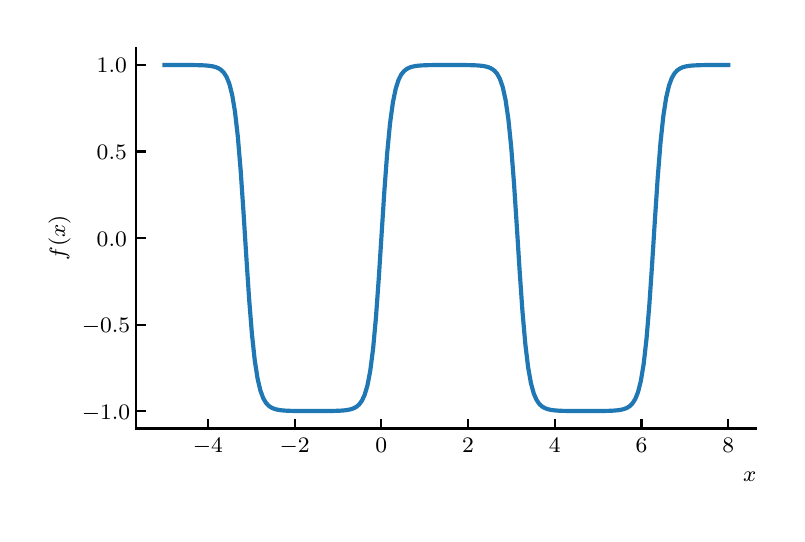
\begin{tikzpicture}%
\node[inner sep=0pt] {%% Creator: Matplotlib, PGF backend
%%
%% To include the figure in your LaTeX document, write
%%   \input{<filename>.pgf}
%%
%% Make sure the required packages are loaded in your preamble
%%   \usepackage{pgf}
%%
%% Also ensure that all the required font packages are loaded; for instance,
%% the lmodern package is sometimes necessary when using math font.
%%   \usepackage{lmodern}
%%
%% Figures using additional raster images can only be included by \input if
%% they are in the same directory as the main LaTeX file. For loading figures
%% from other directories you can use the `import` package
%%   \usepackage{import}
%%
%% and then include the figures with
%%   \import{<path to file>}{<filename>.pgf}
%%
%% Matplotlib used the following preamble
%%   \def\mathdefault#1{#1}
%%   \everymath=\expandafter{\the\everymath\displaystyle}
%%   \RequirePackage[T1]{fontenc}%
%%   \usepackage{newpxmath} % math font is Palatino compatible
%%   \let\Bbbk\relax % so it doesn't clash with amssymb
%%   \usepackage[no-math]{fontspec}
%%   \setmainfont{Palatino}
%%   \setmonofont{Latin Modern Mono}[%
%%   Scale=1.05, % a touch smaller than MatchLowercase
%%   BoldFont=*,
%%   BoldFeatures={FakeBold=2}
%%   ]
%%   \setsansfont{Helvetica}
%%   \renewcommand{\mathdefault}[1][]{}
%%   \usepackage{fontspec}
%%   \setmainfont{Palatino.ttc}[Path=\detokenize{/System/Library/Fonts/}]
%%   \setsansfont{DejaVuSans.ttf}[Path=\detokenize{/Users/ricopicone/anaconda3/envs/engcom/lib/python3.11/site-packages/matplotlib/mpl-data/fonts/ttf/}]
%%   \setmonofont{DejaVuSansMono.ttf}[Path=\detokenize{/Users/ricopicone/anaconda3/envs/engcom/lib/python3.11/site-packages/matplotlib/mpl-data/fonts/ttf/}]
%%   \makeatletter\@ifpackageloaded{underscore}{}{\usepackage[strings]{underscore}}\makeatother
%%
\begingroup%
\makeatletter%
\begin{pgfpicture}%
\pgfpathrectangle{\pgfpointorigin}{\pgfqpoint{3.743499in}{2.430625in}}%
\pgfusepath{use as bounding box, clip}%
\begin{pgfscope}%
\pgfsetbuttcap%
\pgfsetmiterjoin%
\definecolor{currentfill}{rgb}{1.000000,1.000000,1.000000}%
\pgfsetfillcolor{currentfill}%
\pgfsetlinewidth{0.000000pt}%
\definecolor{currentstroke}{rgb}{1.000000,1.000000,1.000000}%
\pgfsetstrokecolor{currentstroke}%
\pgfsetdash{}{0pt}%
\pgfpathmoveto{\pgfqpoint{0.000000in}{-0.000000in}}%
\pgfpathlineto{\pgfqpoint{3.743499in}{-0.000000in}}%
\pgfpathlineto{\pgfqpoint{3.743499in}{2.430625in}}%
\pgfpathlineto{\pgfqpoint{0.000000in}{2.430625in}}%
\pgfpathlineto{\pgfqpoint{0.000000in}{-0.000000in}}%
\pgfpathclose%
\pgfusepath{fill}%
\end{pgfscope}%
\begin{pgfscope}%
\pgfsetbuttcap%
\pgfsetmiterjoin%
\definecolor{currentfill}{rgb}{1.000000,1.000000,1.000000}%
\pgfsetfillcolor{currentfill}%
\pgfsetlinewidth{0.000000pt}%
\definecolor{currentstroke}{rgb}{0.000000,0.000000,0.000000}%
\pgfsetstrokecolor{currentstroke}%
\pgfsetstrokeopacity{0.000000}%
\pgfsetdash{}{0pt}%
\pgfpathmoveto{\pgfqpoint{0.543499in}{0.427040in}}%
\pgfpathlineto{\pgfqpoint{3.643499in}{0.427040in}}%
\pgfpathlineto{\pgfqpoint{3.643499in}{2.330625in}}%
\pgfpathlineto{\pgfqpoint{0.543499in}{2.330625in}}%
\pgfpathlineto{\pgfqpoint{0.543499in}{0.427040in}}%
\pgfpathclose%
\pgfusepath{fill}%
\end{pgfscope}%
\begin{pgfscope}%
\pgfsetbuttcap%
\pgfsetroundjoin%
\definecolor{currentfill}{rgb}{0.000000,0.000000,0.000000}%
\pgfsetfillcolor{currentfill}%
\pgfsetlinewidth{0.803000pt}%
\definecolor{currentstroke}{rgb}{0.000000,0.000000,0.000000}%
\pgfsetstrokecolor{currentstroke}%
\pgfsetdash{}{0pt}%
\pgfsys@defobject{currentmarker}{\pgfqpoint{0.000000in}{0.000000in}}{\pgfqpoint{0.000000in}{0.048611in}}{%
\pgfpathmoveto{\pgfqpoint{0.000000in}{0.000000in}}%
\pgfpathlineto{\pgfqpoint{0.000000in}{0.048611in}}%
\pgfusepath{stroke,fill}%
}%
\begin{pgfscope}%
\pgfsys@transformshift{0.901192in}{0.427040in}%
\pgfsys@useobject{currentmarker}{}%
\end{pgfscope}%
\end{pgfscope}%
\begin{pgfscope}%
\definecolor{textcolor}{rgb}{0.000000,0.000000,0.000000}%
\pgfsetstrokecolor{textcolor}%
\pgfsetfillcolor{textcolor}%
\pgftext[x=0.901192in,y=0.378429in,,top]{\color{textcolor}{\rmfamily\fontsize{8.000000}{9.600000}\selectfont\catcode`\^=\active\def^{\ifmmode\sp\else\^{}\fi}\catcode`\%=\active\def%{\%}$\mathdefault{\ensuremath{-}4}$}}%
\end{pgfscope}%
\begin{pgfscope}%
\pgfsetbuttcap%
\pgfsetroundjoin%
\definecolor{currentfill}{rgb}{0.000000,0.000000,0.000000}%
\pgfsetfillcolor{currentfill}%
\pgfsetlinewidth{0.803000pt}%
\definecolor{currentstroke}{rgb}{0.000000,0.000000,0.000000}%
\pgfsetstrokecolor{currentstroke}%
\pgfsetdash{}{0pt}%
\pgfsys@defobject{currentmarker}{\pgfqpoint{0.000000in}{0.000000in}}{\pgfqpoint{0.000000in}{0.048611in}}{%
\pgfpathmoveto{\pgfqpoint{0.000000in}{0.000000in}}%
\pgfpathlineto{\pgfqpoint{0.000000in}{0.048611in}}%
\pgfusepath{stroke,fill}%
}%
\begin{pgfscope}%
\pgfsys@transformshift{1.334758in}{0.427040in}%
\pgfsys@useobject{currentmarker}{}%
\end{pgfscope}%
\end{pgfscope}%
\begin{pgfscope}%
\definecolor{textcolor}{rgb}{0.000000,0.000000,0.000000}%
\pgfsetstrokecolor{textcolor}%
\pgfsetfillcolor{textcolor}%
\pgftext[x=1.334758in,y=0.378429in,,top]{\color{textcolor}{\rmfamily\fontsize{8.000000}{9.600000}\selectfont\catcode`\^=\active\def^{\ifmmode\sp\else\^{}\fi}\catcode`\%=\active\def%{\%}$\mathdefault{\ensuremath{-}2}$}}%
\end{pgfscope}%
\begin{pgfscope}%
\pgfsetbuttcap%
\pgfsetroundjoin%
\definecolor{currentfill}{rgb}{0.000000,0.000000,0.000000}%
\pgfsetfillcolor{currentfill}%
\pgfsetlinewidth{0.803000pt}%
\definecolor{currentstroke}{rgb}{0.000000,0.000000,0.000000}%
\pgfsetstrokecolor{currentstroke}%
\pgfsetdash{}{0pt}%
\pgfsys@defobject{currentmarker}{\pgfqpoint{0.000000in}{0.000000in}}{\pgfqpoint{0.000000in}{0.048611in}}{%
\pgfpathmoveto{\pgfqpoint{0.000000in}{0.000000in}}%
\pgfpathlineto{\pgfqpoint{0.000000in}{0.048611in}}%
\pgfusepath{stroke,fill}%
}%
\begin{pgfscope}%
\pgfsys@transformshift{1.768325in}{0.427040in}%
\pgfsys@useobject{currentmarker}{}%
\end{pgfscope}%
\end{pgfscope}%
\begin{pgfscope}%
\definecolor{textcolor}{rgb}{0.000000,0.000000,0.000000}%
\pgfsetstrokecolor{textcolor}%
\pgfsetfillcolor{textcolor}%
\pgftext[x=1.768325in,y=0.378429in,,top]{\color{textcolor}{\rmfamily\fontsize{8.000000}{9.600000}\selectfont\catcode`\^=\active\def^{\ifmmode\sp\else\^{}\fi}\catcode`\%=\active\def%{\%}$\mathdefault{0}$}}%
\end{pgfscope}%
\begin{pgfscope}%
\pgfsetbuttcap%
\pgfsetroundjoin%
\definecolor{currentfill}{rgb}{0.000000,0.000000,0.000000}%
\pgfsetfillcolor{currentfill}%
\pgfsetlinewidth{0.803000pt}%
\definecolor{currentstroke}{rgb}{0.000000,0.000000,0.000000}%
\pgfsetstrokecolor{currentstroke}%
\pgfsetdash{}{0pt}%
\pgfsys@defobject{currentmarker}{\pgfqpoint{0.000000in}{0.000000in}}{\pgfqpoint{0.000000in}{0.048611in}}{%
\pgfpathmoveto{\pgfqpoint{0.000000in}{0.000000in}}%
\pgfpathlineto{\pgfqpoint{0.000000in}{0.048611in}}%
\pgfusepath{stroke,fill}%
}%
\begin{pgfscope}%
\pgfsys@transformshift{2.201891in}{0.427040in}%
\pgfsys@useobject{currentmarker}{}%
\end{pgfscope}%
\end{pgfscope}%
\begin{pgfscope}%
\definecolor{textcolor}{rgb}{0.000000,0.000000,0.000000}%
\pgfsetstrokecolor{textcolor}%
\pgfsetfillcolor{textcolor}%
\pgftext[x=2.201891in,y=0.378429in,,top]{\color{textcolor}{\rmfamily\fontsize{8.000000}{9.600000}\selectfont\catcode`\^=\active\def^{\ifmmode\sp\else\^{}\fi}\catcode`\%=\active\def%{\%}$\mathdefault{2}$}}%
\end{pgfscope}%
\begin{pgfscope}%
\pgfsetbuttcap%
\pgfsetroundjoin%
\definecolor{currentfill}{rgb}{0.000000,0.000000,0.000000}%
\pgfsetfillcolor{currentfill}%
\pgfsetlinewidth{0.803000pt}%
\definecolor{currentstroke}{rgb}{0.000000,0.000000,0.000000}%
\pgfsetstrokecolor{currentstroke}%
\pgfsetdash{}{0pt}%
\pgfsys@defobject{currentmarker}{\pgfqpoint{0.000000in}{0.000000in}}{\pgfqpoint{0.000000in}{0.048611in}}{%
\pgfpathmoveto{\pgfqpoint{0.000000in}{0.000000in}}%
\pgfpathlineto{\pgfqpoint{0.000000in}{0.048611in}}%
\pgfusepath{stroke,fill}%
}%
\begin{pgfscope}%
\pgfsys@transformshift{2.635457in}{0.427040in}%
\pgfsys@useobject{currentmarker}{}%
\end{pgfscope}%
\end{pgfscope}%
\begin{pgfscope}%
\definecolor{textcolor}{rgb}{0.000000,0.000000,0.000000}%
\pgfsetstrokecolor{textcolor}%
\pgfsetfillcolor{textcolor}%
\pgftext[x=2.635457in,y=0.378429in,,top]{\color{textcolor}{\rmfamily\fontsize{8.000000}{9.600000}\selectfont\catcode`\^=\active\def^{\ifmmode\sp\else\^{}\fi}\catcode`\%=\active\def%{\%}$\mathdefault{4}$}}%
\end{pgfscope}%
\begin{pgfscope}%
\pgfsetbuttcap%
\pgfsetroundjoin%
\definecolor{currentfill}{rgb}{0.000000,0.000000,0.000000}%
\pgfsetfillcolor{currentfill}%
\pgfsetlinewidth{0.803000pt}%
\definecolor{currentstroke}{rgb}{0.000000,0.000000,0.000000}%
\pgfsetstrokecolor{currentstroke}%
\pgfsetdash{}{0pt}%
\pgfsys@defobject{currentmarker}{\pgfqpoint{0.000000in}{0.000000in}}{\pgfqpoint{0.000000in}{0.048611in}}{%
\pgfpathmoveto{\pgfqpoint{0.000000in}{0.000000in}}%
\pgfpathlineto{\pgfqpoint{0.000000in}{0.048611in}}%
\pgfusepath{stroke,fill}%
}%
\begin{pgfscope}%
\pgfsys@transformshift{3.069024in}{0.427040in}%
\pgfsys@useobject{currentmarker}{}%
\end{pgfscope}%
\end{pgfscope}%
\begin{pgfscope}%
\definecolor{textcolor}{rgb}{0.000000,0.000000,0.000000}%
\pgfsetstrokecolor{textcolor}%
\pgfsetfillcolor{textcolor}%
\pgftext[x=3.069024in,y=0.378429in,,top]{\color{textcolor}{\rmfamily\fontsize{8.000000}{9.600000}\selectfont\catcode`\^=\active\def^{\ifmmode\sp\else\^{}\fi}\catcode`\%=\active\def%{\%}$\mathdefault{6}$}}%
\end{pgfscope}%
\begin{pgfscope}%
\pgfsetbuttcap%
\pgfsetroundjoin%
\definecolor{currentfill}{rgb}{0.000000,0.000000,0.000000}%
\pgfsetfillcolor{currentfill}%
\pgfsetlinewidth{0.803000pt}%
\definecolor{currentstroke}{rgb}{0.000000,0.000000,0.000000}%
\pgfsetstrokecolor{currentstroke}%
\pgfsetdash{}{0pt}%
\pgfsys@defobject{currentmarker}{\pgfqpoint{0.000000in}{0.000000in}}{\pgfqpoint{0.000000in}{0.048611in}}{%
\pgfpathmoveto{\pgfqpoint{0.000000in}{0.000000in}}%
\pgfpathlineto{\pgfqpoint{0.000000in}{0.048611in}}%
\pgfusepath{stroke,fill}%
}%
\begin{pgfscope}%
\pgfsys@transformshift{3.502590in}{0.427040in}%
\pgfsys@useobject{currentmarker}{}%
\end{pgfscope}%
\end{pgfscope}%
\begin{pgfscope}%
\definecolor{textcolor}{rgb}{0.000000,0.000000,0.000000}%
\pgfsetstrokecolor{textcolor}%
\pgfsetfillcolor{textcolor}%
\pgftext[x=3.502590in,y=0.378429in,,top]{\color{textcolor}{\rmfamily\fontsize{8.000000}{9.600000}\selectfont\catcode`\^=\active\def^{\ifmmode\sp\else\^{}\fi}\catcode`\%=\active\def%{\%}$\mathdefault{8}$}}%
\end{pgfscope}%
\begin{pgfscope}%
\definecolor{textcolor}{rgb}{0.000000,0.000000,0.000000}%
\pgfsetstrokecolor{textcolor}%
\pgfsetfillcolor{textcolor}%
\pgftext[x=3.643499in,y=0.211437in,right,top]{\color{textcolor}{\rmfamily\fontsize{8.000000}{9.600000}\selectfont\catcode`\^=\active\def^{\ifmmode\sp\else\^{}\fi}\catcode`\%=\active\def%{\%}$x$}}%
\end{pgfscope}%
\begin{pgfscope}%
\pgfsetbuttcap%
\pgfsetroundjoin%
\definecolor{currentfill}{rgb}{0.000000,0.000000,0.000000}%
\pgfsetfillcolor{currentfill}%
\pgfsetlinewidth{0.803000pt}%
\definecolor{currentstroke}{rgb}{0.000000,0.000000,0.000000}%
\pgfsetstrokecolor{currentstroke}%
\pgfsetdash{}{0pt}%
\pgfsys@defobject{currentmarker}{\pgfqpoint{0.000000in}{0.000000in}}{\pgfqpoint{0.048611in}{0.000000in}}{%
\pgfpathmoveto{\pgfqpoint{0.000000in}{0.000000in}}%
\pgfpathlineto{\pgfqpoint{0.048611in}{0.000000in}}%
\pgfusepath{stroke,fill}%
}%
\begin{pgfscope}%
\pgfsys@transformshift{0.543499in}{0.512985in}%
\pgfsys@useobject{currentmarker}{}%
\end{pgfscope}%
\end{pgfscope}%
\begin{pgfscope}%
\definecolor{textcolor}{rgb}{0.000000,0.000000,0.000000}%
\pgfsetstrokecolor{textcolor}%
\pgfsetfillcolor{textcolor}%
\pgftext[x=0.271055in, y=0.472566in, left, base]{\color{textcolor}{\rmfamily\fontsize{8.000000}{9.600000}\selectfont\catcode`\^=\active\def^{\ifmmode\sp\else\^{}\fi}\catcode`\%=\active\def%{\%}$\mathdefault{\ensuremath{-}1.0}$}}%
\end{pgfscope}%
\begin{pgfscope}%
\pgfsetbuttcap%
\pgfsetroundjoin%
\definecolor{currentfill}{rgb}{0.000000,0.000000,0.000000}%
\pgfsetfillcolor{currentfill}%
\pgfsetlinewidth{0.803000pt}%
\definecolor{currentstroke}{rgb}{0.000000,0.000000,0.000000}%
\pgfsetstrokecolor{currentstroke}%
\pgfsetdash{}{0pt}%
\pgfsys@defobject{currentmarker}{\pgfqpoint{0.000000in}{0.000000in}}{\pgfqpoint{0.048611in}{0.000000in}}{%
\pgfpathmoveto{\pgfqpoint{0.000000in}{0.000000in}}%
\pgfpathlineto{\pgfqpoint{0.048611in}{0.000000in}}%
\pgfusepath{stroke,fill}%
}%
\begin{pgfscope}%
\pgfsys@transformshift{0.543499in}{0.945909in}%
\pgfsys@useobject{currentmarker}{}%
\end{pgfscope}%
\end{pgfscope}%
\begin{pgfscope}%
\definecolor{textcolor}{rgb}{0.000000,0.000000,0.000000}%
\pgfsetstrokecolor{textcolor}%
\pgfsetfillcolor{textcolor}%
\pgftext[x=0.271055in, y=0.905490in, left, base]{\color{textcolor}{\rmfamily\fontsize{8.000000}{9.600000}\selectfont\catcode`\^=\active\def^{\ifmmode\sp\else\^{}\fi}\catcode`\%=\active\def%{\%}$\mathdefault{\ensuremath{-}0.5}$}}%
\end{pgfscope}%
\begin{pgfscope}%
\pgfsetbuttcap%
\pgfsetroundjoin%
\definecolor{currentfill}{rgb}{0.000000,0.000000,0.000000}%
\pgfsetfillcolor{currentfill}%
\pgfsetlinewidth{0.803000pt}%
\definecolor{currentstroke}{rgb}{0.000000,0.000000,0.000000}%
\pgfsetstrokecolor{currentstroke}%
\pgfsetdash{}{0pt}%
\pgfsys@defobject{currentmarker}{\pgfqpoint{0.000000in}{0.000000in}}{\pgfqpoint{0.048611in}{0.000000in}}{%
\pgfpathmoveto{\pgfqpoint{0.000000in}{0.000000in}}%
\pgfpathlineto{\pgfqpoint{0.048611in}{0.000000in}}%
\pgfusepath{stroke,fill}%
}%
\begin{pgfscope}%
\pgfsys@transformshift{0.543499in}{1.378832in}%
\pgfsys@useobject{currentmarker}{}%
\end{pgfscope}%
\end{pgfscope}%
\begin{pgfscope}%
\definecolor{textcolor}{rgb}{0.000000,0.000000,0.000000}%
\pgfsetstrokecolor{textcolor}%
\pgfsetfillcolor{textcolor}%
\pgftext[x=0.345388in, y=1.338413in, left, base]{\color{textcolor}{\rmfamily\fontsize{8.000000}{9.600000}\selectfont\catcode`\^=\active\def^{\ifmmode\sp\else\^{}\fi}\catcode`\%=\active\def%{\%}$\mathdefault{0.0}$}}%
\end{pgfscope}%
\begin{pgfscope}%
\pgfsetbuttcap%
\pgfsetroundjoin%
\definecolor{currentfill}{rgb}{0.000000,0.000000,0.000000}%
\pgfsetfillcolor{currentfill}%
\pgfsetlinewidth{0.803000pt}%
\definecolor{currentstroke}{rgb}{0.000000,0.000000,0.000000}%
\pgfsetstrokecolor{currentstroke}%
\pgfsetdash{}{0pt}%
\pgfsys@defobject{currentmarker}{\pgfqpoint{0.000000in}{0.000000in}}{\pgfqpoint{0.048611in}{0.000000in}}{%
\pgfpathmoveto{\pgfqpoint{0.000000in}{0.000000in}}%
\pgfpathlineto{\pgfqpoint{0.048611in}{0.000000in}}%
\pgfusepath{stroke,fill}%
}%
\begin{pgfscope}%
\pgfsys@transformshift{0.543499in}{1.811755in}%
\pgfsys@useobject{currentmarker}{}%
\end{pgfscope}%
\end{pgfscope}%
\begin{pgfscope}%
\definecolor{textcolor}{rgb}{0.000000,0.000000,0.000000}%
\pgfsetstrokecolor{textcolor}%
\pgfsetfillcolor{textcolor}%
\pgftext[x=0.345388in, y=1.771337in, left, base]{\color{textcolor}{\rmfamily\fontsize{8.000000}{9.600000}\selectfont\catcode`\^=\active\def^{\ifmmode\sp\else\^{}\fi}\catcode`\%=\active\def%{\%}$\mathdefault{0.5}$}}%
\end{pgfscope}%
\begin{pgfscope}%
\pgfsetbuttcap%
\pgfsetroundjoin%
\definecolor{currentfill}{rgb}{0.000000,0.000000,0.000000}%
\pgfsetfillcolor{currentfill}%
\pgfsetlinewidth{0.803000pt}%
\definecolor{currentstroke}{rgb}{0.000000,0.000000,0.000000}%
\pgfsetstrokecolor{currentstroke}%
\pgfsetdash{}{0pt}%
\pgfsys@defobject{currentmarker}{\pgfqpoint{0.000000in}{0.000000in}}{\pgfqpoint{0.048611in}{0.000000in}}{%
\pgfpathmoveto{\pgfqpoint{0.000000in}{0.000000in}}%
\pgfpathlineto{\pgfqpoint{0.048611in}{0.000000in}}%
\pgfusepath{stroke,fill}%
}%
\begin{pgfscope}%
\pgfsys@transformshift{0.543499in}{2.244679in}%
\pgfsys@useobject{currentmarker}{}%
\end{pgfscope}%
\end{pgfscope}%
\begin{pgfscope}%
\definecolor{textcolor}{rgb}{0.000000,0.000000,0.000000}%
\pgfsetstrokecolor{textcolor}%
\pgfsetfillcolor{textcolor}%
\pgftext[x=0.345388in, y=2.204260in, left, base]{\color{textcolor}{\rmfamily\fontsize{8.000000}{9.600000}\selectfont\catcode`\^=\active\def^{\ifmmode\sp\else\^{}\fi}\catcode`\%=\active\def%{\%}$\mathdefault{1.0}$}}%
\end{pgfscope}%
\begin{pgfscope}%
\definecolor{textcolor}{rgb}{0.000000,0.000000,0.000000}%
\pgfsetstrokecolor{textcolor}%
\pgfsetfillcolor{textcolor}%
\pgftext[x=0.215500in,y=1.378832in,,bottom,rotate=90.000000]{\color{textcolor}{\rmfamily\fontsize{8.000000}{9.600000}\selectfont\catcode`\^=\active\def^{\ifmmode\sp\else\^{}\fi}\catcode`\%=\active\def%{\%}$f(x)$}}%
\end{pgfscope}%
\begin{pgfscope}%
\pgfpathrectangle{\pgfqpoint{0.543499in}{0.427040in}}{\pgfqpoint{3.100000in}{1.903585in}}%
\pgfusepath{clip}%
\pgfsetrectcap%
\pgfsetroundjoin%
\pgfsetlinewidth{1.505625pt}%
\definecolor{currentstroke}{rgb}{0.121569,0.466667,0.705882}%
\pgfsetstrokecolor{currentstroke}%
\pgfsetdash{}{0pt}%
\pgfpathmoveto{\pgfqpoint{0.684409in}{2.243872in}}%
\pgfpathlineto{\pgfqpoint{0.740772in}{2.244096in}}%
\pgfpathlineto{\pgfqpoint{0.797136in}{2.243959in}}%
\pgfpathlineto{\pgfqpoint{0.839409in}{2.243487in}}%
\pgfpathlineto{\pgfqpoint{0.867590in}{2.242731in}}%
\pgfpathlineto{\pgfqpoint{0.881681in}{2.242079in}}%
\pgfpathlineto{\pgfqpoint{0.895772in}{2.241113in}}%
\pgfpathlineto{\pgfqpoint{0.909863in}{2.239659in}}%
\pgfpathlineto{\pgfqpoint{0.923954in}{2.237439in}}%
\pgfpathlineto{\pgfqpoint{0.938045in}{2.234001in}}%
\pgfpathlineto{\pgfqpoint{0.952136in}{2.228607in}}%
\pgfpathlineto{\pgfqpoint{0.966227in}{2.220052in}}%
\pgfpathlineto{\pgfqpoint{0.980318in}{2.206379in}}%
\pgfpathlineto{\pgfqpoint{0.994409in}{2.184455in}}%
\pgfpathlineto{\pgfqpoint{1.008499in}{2.149421in}}%
\pgfpathlineto{\pgfqpoint{1.022590in}{2.094181in}}%
\pgfpathlineto{\pgfqpoint{1.036681in}{2.009460in}}%
\pgfpathlineto{\pgfqpoint{1.050772in}{1.885591in}}%
\pgfpathlineto{\pgfqpoint{1.064863in}{1.717314in}}%
\pgfpathlineto{\pgfqpoint{1.078954in}{1.510783in}}%
\pgfpathlineto{\pgfqpoint{1.093045in}{1.287088in}}%
\pgfpathlineto{\pgfqpoint{1.107136in}{1.075471in}}%
\pgfpathlineto{\pgfqpoint{1.121227in}{0.899345in}}%
\pgfpathlineto{\pgfqpoint{1.135318in}{0.767557in}}%
\pgfpathlineto{\pgfqpoint{1.149409in}{0.676394in}}%
\pgfpathlineto{\pgfqpoint{1.163499in}{0.616535in}}%
\pgfpathlineto{\pgfqpoint{1.177590in}{0.578427in}}%
\pgfpathlineto{\pgfqpoint{1.191681in}{0.554541in}}%
\pgfpathlineto{\pgfqpoint{1.205772in}{0.539644in}}%
\pgfpathlineto{\pgfqpoint{1.219863in}{0.530332in}}%
\pgfpathlineto{\pgfqpoint{1.233954in}{0.524471in}}%
\pgfpathlineto{\pgfqpoint{1.248045in}{0.520743in}}%
\pgfpathlineto{\pgfqpoint{1.262136in}{0.518342in}}%
\pgfpathlineto{\pgfqpoint{1.276227in}{0.516773in}}%
\pgfpathlineto{\pgfqpoint{1.290318in}{0.515733in}}%
\pgfpathlineto{\pgfqpoint{1.304409in}{0.515034in}}%
\pgfpathlineto{\pgfqpoint{1.332590in}{0.514226in}}%
\pgfpathlineto{\pgfqpoint{1.360772in}{0.513834in}}%
\pgfpathlineto{\pgfqpoint{1.403045in}{0.513597in}}%
\pgfpathlineto{\pgfqpoint{1.459409in}{0.513617in}}%
\pgfpathlineto{\pgfqpoint{1.501681in}{0.513905in}}%
\pgfpathlineto{\pgfqpoint{1.529863in}{0.514371in}}%
\pgfpathlineto{\pgfqpoint{1.558045in}{0.515340in}}%
\pgfpathlineto{\pgfqpoint{1.572136in}{0.516187in}}%
\pgfpathlineto{\pgfqpoint{1.586227in}{0.517454in}}%
\pgfpathlineto{\pgfqpoint{1.600318in}{0.519380in}}%
\pgfpathlineto{\pgfqpoint{1.614409in}{0.522348in}}%
\pgfpathlineto{\pgfqpoint{1.628499in}{0.526987in}}%
\pgfpathlineto{\pgfqpoint{1.642590in}{0.534319in}}%
\pgfpathlineto{\pgfqpoint{1.656681in}{0.546012in}}%
\pgfpathlineto{\pgfqpoint{1.670772in}{0.564754in}}%
\pgfpathlineto{\pgfqpoint{1.684863in}{0.594763in}}%
\pgfpathlineto{\pgfqpoint{1.698954in}{0.642355in}}%
\pgfpathlineto{\pgfqpoint{1.713045in}{0.716164in}}%
\pgfpathlineto{\pgfqpoint{1.727136in}{0.826092in}}%
\pgfpathlineto{\pgfqpoint{1.741227in}{0.979596in}}%
\pgfpathlineto{\pgfqpoint{1.755318in}{1.175047in}}%
\pgfpathlineto{\pgfqpoint{1.783499in}{1.614943in}}%
\pgfpathlineto{\pgfqpoint{1.797590in}{1.804609in}}%
\pgfpathlineto{\pgfqpoint{1.811681in}{1.951201in}}%
\pgfpathlineto{\pgfqpoint{1.825772in}{2.054960in}}%
\pgfpathlineto{\pgfqpoint{1.839863in}{2.124096in}}%
\pgfpathlineto{\pgfqpoint{1.853954in}{2.168477in}}%
\pgfpathlineto{\pgfqpoint{1.868045in}{2.196400in}}%
\pgfpathlineto{\pgfqpoint{1.882136in}{2.213828in}}%
\pgfpathlineto{\pgfqpoint{1.896227in}{2.224706in}}%
\pgfpathlineto{\pgfqpoint{1.910318in}{2.231535in}}%
\pgfpathlineto{\pgfqpoint{1.924409in}{2.235862in}}%
\pgfpathlineto{\pgfqpoint{1.938499in}{2.238637in}}%
\pgfpathlineto{\pgfqpoint{1.952590in}{2.240441in}}%
\pgfpathlineto{\pgfqpoint{1.966681in}{2.241631in}}%
\pgfpathlineto{\pgfqpoint{1.980772in}{2.242427in}}%
\pgfpathlineto{\pgfqpoint{2.008954in}{2.243342in}}%
\pgfpathlineto{\pgfqpoint{2.037136in}{2.243783in}}%
\pgfpathlineto{\pgfqpoint{2.079409in}{2.244054in}}%
\pgfpathlineto{\pgfqpoint{2.135772in}{2.244061in}}%
\pgfpathlineto{\pgfqpoint{2.178045in}{2.243809in}}%
\pgfpathlineto{\pgfqpoint{2.206227in}{2.243395in}}%
\pgfpathlineto{\pgfqpoint{2.234409in}{2.242540in}}%
\pgfpathlineto{\pgfqpoint{2.248499in}{2.241797in}}%
\pgfpathlineto{\pgfqpoint{2.262590in}{2.240690in}}%
\pgfpathlineto{\pgfqpoint{2.276681in}{2.239017in}}%
\pgfpathlineto{\pgfqpoint{2.290772in}{2.236450in}}%
\pgfpathlineto{\pgfqpoint{2.304863in}{2.232456in}}%
\pgfpathlineto{\pgfqpoint{2.318954in}{2.226166in}}%
\pgfpathlineto{\pgfqpoint{2.333045in}{2.216160in}}%
\pgfpathlineto{\pgfqpoint{2.347136in}{2.200140in}}%
\pgfpathlineto{\pgfqpoint{2.361227in}{2.174461in}}%
\pgfpathlineto{\pgfqpoint{2.375318in}{2.133557in}}%
\pgfpathlineto{\pgfqpoint{2.389409in}{2.069538in}}%
\pgfpathlineto{\pgfqpoint{2.403499in}{1.972669in}}%
\pgfpathlineto{\pgfqpoint{2.417590in}{1.834063in}}%
\pgfpathlineto{\pgfqpoint{2.431681in}{1.651513in}}%
\pgfpathlineto{\pgfqpoint{2.445772in}{1.436212in}}%
\pgfpathlineto{\pgfqpoint{2.459863in}{1.213306in}}%
\pgfpathlineto{\pgfqpoint{2.473954in}{1.011643in}}%
\pgfpathlineto{\pgfqpoint{2.488045in}{0.850161in}}%
\pgfpathlineto{\pgfqpoint{2.502136in}{0.732845in}}%
\pgfpathlineto{\pgfqpoint{2.516227in}{0.653318in}}%
\pgfpathlineto{\pgfqpoint{2.530318in}{0.601744in}}%
\pgfpathlineto{\pgfqpoint{2.544409in}{0.569129in}}%
\pgfpathlineto{\pgfqpoint{2.558499in}{0.548740in}}%
\pgfpathlineto{\pgfqpoint{2.572590in}{0.536023in}}%
\pgfpathlineto{\pgfqpoint{2.586681in}{0.528059in}}%
\pgfpathlineto{\pgfqpoint{2.600772in}{0.523030in}}%
\pgfpathlineto{\pgfqpoint{2.614863in}{0.519819in}}%
\pgfpathlineto{\pgfqpoint{2.628954in}{0.517741in}}%
\pgfpathlineto{\pgfqpoint{2.643045in}{0.516377in}}%
\pgfpathlineto{\pgfqpoint{2.657136in}{0.515468in}}%
\pgfpathlineto{\pgfqpoint{2.671227in}{0.514853in}}%
\pgfpathlineto{\pgfqpoint{2.699409in}{0.514139in}}%
\pgfpathlineto{\pgfqpoint{2.741681in}{0.513692in}}%
\pgfpathlineto{\pgfqpoint{2.798045in}{0.513569in}}%
\pgfpathlineto{\pgfqpoint{2.854409in}{0.513811in}}%
\pgfpathlineto{\pgfqpoint{2.882590in}{0.514178in}}%
\pgfpathlineto{\pgfqpoint{2.910772in}{0.514935in}}%
\pgfpathlineto{\pgfqpoint{2.924863in}{0.515588in}}%
\pgfpathlineto{\pgfqpoint{2.938954in}{0.516556in}}%
\pgfpathlineto{\pgfqpoint{2.953045in}{0.518012in}}%
\pgfpathlineto{\pgfqpoint{2.967136in}{0.520235in}}%
\pgfpathlineto{\pgfqpoint{2.981227in}{0.523678in}}%
\pgfpathlineto{\pgfqpoint{2.995318in}{0.529080in}}%
\pgfpathlineto{\pgfqpoint{3.009409in}{0.537649in}}%
\pgfpathlineto{\pgfqpoint{3.023499in}{0.551344in}}%
\pgfpathlineto{\pgfqpoint{3.037590in}{0.573304in}}%
\pgfpathlineto{\pgfqpoint{3.051681in}{0.608393in}}%
\pgfpathlineto{\pgfqpoint{3.065772in}{0.663717in}}%
\pgfpathlineto{\pgfqpoint{3.079863in}{0.748556in}}%
\pgfpathlineto{\pgfqpoint{3.093954in}{0.872572in}}%
\pgfpathlineto{\pgfqpoint{3.108045in}{1.040998in}}%
\pgfpathlineto{\pgfqpoint{3.122136in}{1.247632in}}%
\pgfpathlineto{\pgfqpoint{3.136227in}{1.471336in}}%
\pgfpathlineto{\pgfqpoint{3.150318in}{1.682865in}}%
\pgfpathlineto{\pgfqpoint{3.164409in}{1.858845in}}%
\pgfpathlineto{\pgfqpoint{3.178499in}{1.990483in}}%
\pgfpathlineto{\pgfqpoint{3.192590in}{2.081522in}}%
\pgfpathlineto{\pgfqpoint{3.206681in}{2.141292in}}%
\pgfpathlineto{\pgfqpoint{3.220772in}{2.179340in}}%
\pgfpathlineto{\pgfqpoint{3.234863in}{2.203187in}}%
\pgfpathlineto{\pgfqpoint{3.248954in}{2.218060in}}%
\pgfpathlineto{\pgfqpoint{3.263045in}{2.227357in}}%
\pgfpathlineto{\pgfqpoint{3.277136in}{2.233209in}}%
\pgfpathlineto{\pgfqpoint{3.291227in}{2.236932in}}%
\pgfpathlineto{\pgfqpoint{3.305318in}{2.239329in}}%
\pgfpathlineto{\pgfqpoint{3.319409in}{2.240895in}}%
\pgfpathlineto{\pgfqpoint{3.333499in}{2.241934in}}%
\pgfpathlineto{\pgfqpoint{3.347590in}{2.242633in}}%
\pgfpathlineto{\pgfqpoint{3.375772in}{2.243439in}}%
\pgfpathlineto{\pgfqpoint{3.403954in}{2.243831in}}%
\pgfpathlineto{\pgfqpoint{3.446227in}{2.244067in}}%
\pgfpathlineto{\pgfqpoint{3.502590in}{2.244047in}}%
\pgfpathlineto{\pgfqpoint{3.502590in}{2.244047in}}%
\pgfusepath{stroke}%
\end{pgfscope}%
\begin{pgfscope}%
\pgfsetrectcap%
\pgfsetmiterjoin%
\pgfsetlinewidth{0.803000pt}%
\definecolor{currentstroke}{rgb}{0.000000,0.000000,0.000000}%
\pgfsetstrokecolor{currentstroke}%
\pgfsetdash{}{0pt}%
\pgfpathmoveto{\pgfqpoint{0.543499in}{0.427040in}}%
\pgfpathlineto{\pgfqpoint{0.543499in}{2.330625in}}%
\pgfusepath{stroke}%
\end{pgfscope}%
\begin{pgfscope}%
\pgfsetrectcap%
\pgfsetmiterjoin%
\pgfsetlinewidth{0.803000pt}%
\definecolor{currentstroke}{rgb}{0.000000,0.000000,0.000000}%
\pgfsetstrokecolor{currentstroke}%
\pgfsetdash{}{0pt}%
\pgfpathmoveto{\pgfqpoint{0.543499in}{0.427040in}}%
\pgfpathlineto{\pgfqpoint{3.643499in}{0.427040in}}%
\pgfusepath{stroke}%
\end{pgfscope}%
\end{pgfpicture}%
\makeatother%
\endgroup%
};%
\end{tikzpicture}%
\caption{}
\label{fig:publishing_with_makefile-figure-0}
\end{figure}

\phantomsection\label{e88b3fb7}
Plot $g(x)$:

\phantomsection\label{2ea0e5e8}
\nointerlineskip\nointerlineskip\begin{minted}[autogobble,samepage]{python}
fig, ax = plt.subplots()
plotter(fig, fun=g, limits=(0, 100), labels=("$x$", "$g(x)$"))
\end{minted}

\phantomsection\label{d4d0c3be}
\gdef\graphicslist{}%
\begin{figure}[htbp]
\centering
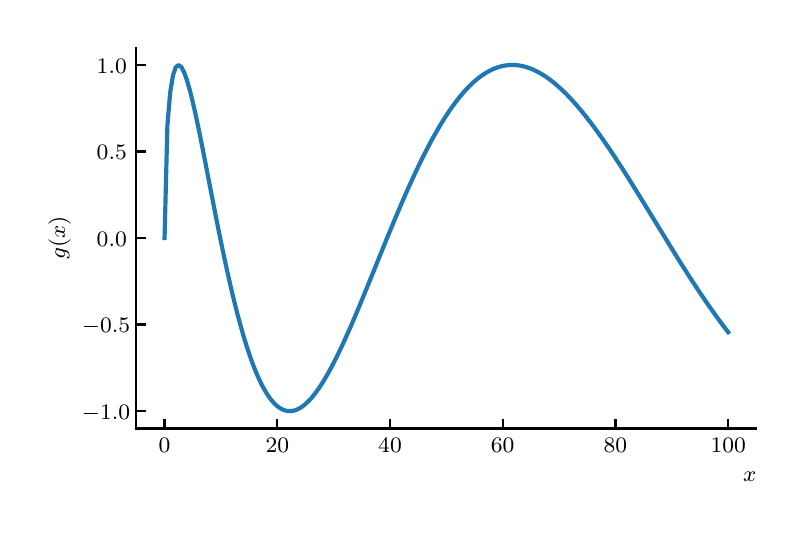
\begin{tikzpicture}%
\node[inner sep=0pt] {%% Creator: Matplotlib, PGF backend
%%
%% To include the figure in your LaTeX document, write
%%   \input{<filename>.pgf}
%%
%% Make sure the required packages are loaded in your preamble
%%   \usepackage{pgf}
%%
%% Also ensure that all the required font packages are loaded; for instance,
%% the lmodern package is sometimes necessary when using math font.
%%   \usepackage{lmodern}
%%
%% Figures using additional raster images can only be included by \input if
%% they are in the same directory as the main LaTeX file. For loading figures
%% from other directories you can use the `import` package
%%   \usepackage{import}
%%
%% and then include the figures with
%%   \import{<path to file>}{<filename>.pgf}
%%
%% Matplotlib used the following preamble
%%   \def\mathdefault#1{#1}
%%   \everymath=\expandafter{\the\everymath\displaystyle}
%%   \RequirePackage[T1]{fontenc}%
%%   \usepackage{newpxmath} % math font is Palatino compatible
%%   \let\Bbbk\relax % so it doesn't clash with amssymb
%%   \usepackage[no-math]{fontspec}
%%   \setmainfont{Palatino}
%%   \setmonofont{Latin Modern Mono}[%
%%   Scale=1.05, % a touch smaller than MatchLowercase
%%   BoldFont=*,
%%   BoldFeatures={FakeBold=2}
%%   ]
%%   \setsansfont{Helvetica}
%%   \renewcommand{\mathdefault}[1][]{}
%%   \usepackage{fontspec}
%%   \setmainfont{Palatino.ttc}[Path=\detokenize{/System/Library/Fonts/}]
%%   \setsansfont{DejaVuSans.ttf}[Path=\detokenize{/Users/ricopicone/anaconda3/envs/engcom/lib/python3.11/site-packages/matplotlib/mpl-data/fonts/ttf/}]
%%   \setmonofont{DejaVuSansMono.ttf}[Path=\detokenize{/Users/ricopicone/anaconda3/envs/engcom/lib/python3.11/site-packages/matplotlib/mpl-data/fonts/ttf/}]
%%   \makeatletter\@ifpackageloaded{underscore}{}{\usepackage[strings]{underscore}}\makeatother
%%
\begingroup%
\makeatletter%
\begin{pgfpicture}%
\pgfpathrectangle{\pgfpointorigin}{\pgfqpoint{3.743499in}{2.430625in}}%
\pgfusepath{use as bounding box, clip}%
\begin{pgfscope}%
\pgfsetbuttcap%
\pgfsetmiterjoin%
\definecolor{currentfill}{rgb}{1.000000,1.000000,1.000000}%
\pgfsetfillcolor{currentfill}%
\pgfsetlinewidth{0.000000pt}%
\definecolor{currentstroke}{rgb}{1.000000,1.000000,1.000000}%
\pgfsetstrokecolor{currentstroke}%
\pgfsetdash{}{0pt}%
\pgfpathmoveto{\pgfqpoint{0.000000in}{-0.000000in}}%
\pgfpathlineto{\pgfqpoint{3.743499in}{-0.000000in}}%
\pgfpathlineto{\pgfqpoint{3.743499in}{2.430625in}}%
\pgfpathlineto{\pgfqpoint{0.000000in}{2.430625in}}%
\pgfpathlineto{\pgfqpoint{0.000000in}{-0.000000in}}%
\pgfpathclose%
\pgfusepath{fill}%
\end{pgfscope}%
\begin{pgfscope}%
\pgfsetbuttcap%
\pgfsetmiterjoin%
\definecolor{currentfill}{rgb}{1.000000,1.000000,1.000000}%
\pgfsetfillcolor{currentfill}%
\pgfsetlinewidth{0.000000pt}%
\definecolor{currentstroke}{rgb}{0.000000,0.000000,0.000000}%
\pgfsetstrokecolor{currentstroke}%
\pgfsetstrokeopacity{0.000000}%
\pgfsetdash{}{0pt}%
\pgfpathmoveto{\pgfqpoint{0.543499in}{0.427040in}}%
\pgfpathlineto{\pgfqpoint{3.643499in}{0.427040in}}%
\pgfpathlineto{\pgfqpoint{3.643499in}{2.330625in}}%
\pgfpathlineto{\pgfqpoint{0.543499in}{2.330625in}}%
\pgfpathlineto{\pgfqpoint{0.543499in}{0.427040in}}%
\pgfpathclose%
\pgfusepath{fill}%
\end{pgfscope}%
\begin{pgfscope}%
\pgfsetbuttcap%
\pgfsetroundjoin%
\definecolor{currentfill}{rgb}{0.000000,0.000000,0.000000}%
\pgfsetfillcolor{currentfill}%
\pgfsetlinewidth{0.803000pt}%
\definecolor{currentstroke}{rgb}{0.000000,0.000000,0.000000}%
\pgfsetstrokecolor{currentstroke}%
\pgfsetdash{}{0pt}%
\pgfsys@defobject{currentmarker}{\pgfqpoint{0.000000in}{0.000000in}}{\pgfqpoint{0.000000in}{0.048611in}}{%
\pgfpathmoveto{\pgfqpoint{0.000000in}{0.000000in}}%
\pgfpathlineto{\pgfqpoint{0.000000in}{0.048611in}}%
\pgfusepath{stroke,fill}%
}%
\begin{pgfscope}%
\pgfsys@transformshift{0.684409in}{0.427040in}%
\pgfsys@useobject{currentmarker}{}%
\end{pgfscope}%
\end{pgfscope}%
\begin{pgfscope}%
\definecolor{textcolor}{rgb}{0.000000,0.000000,0.000000}%
\pgfsetstrokecolor{textcolor}%
\pgfsetfillcolor{textcolor}%
\pgftext[x=0.684409in,y=0.378429in,,top]{\color{textcolor}{\rmfamily\fontsize{8.000000}{9.600000}\selectfont\catcode`\^=\active\def^{\ifmmode\sp\else\^{}\fi}\catcode`\%=\active\def%{\%}$\mathdefault{0}$}}%
\end{pgfscope}%
\begin{pgfscope}%
\pgfsetbuttcap%
\pgfsetroundjoin%
\definecolor{currentfill}{rgb}{0.000000,0.000000,0.000000}%
\pgfsetfillcolor{currentfill}%
\pgfsetlinewidth{0.803000pt}%
\definecolor{currentstroke}{rgb}{0.000000,0.000000,0.000000}%
\pgfsetstrokecolor{currentstroke}%
\pgfsetdash{}{0pt}%
\pgfsys@defobject{currentmarker}{\pgfqpoint{0.000000in}{0.000000in}}{\pgfqpoint{0.000000in}{0.048611in}}{%
\pgfpathmoveto{\pgfqpoint{0.000000in}{0.000000in}}%
\pgfpathlineto{\pgfqpoint{0.000000in}{0.048611in}}%
\pgfusepath{stroke,fill}%
}%
\begin{pgfscope}%
\pgfsys@transformshift{1.248045in}{0.427040in}%
\pgfsys@useobject{currentmarker}{}%
\end{pgfscope}%
\end{pgfscope}%
\begin{pgfscope}%
\definecolor{textcolor}{rgb}{0.000000,0.000000,0.000000}%
\pgfsetstrokecolor{textcolor}%
\pgfsetfillcolor{textcolor}%
\pgftext[x=1.248045in,y=0.378429in,,top]{\color{textcolor}{\rmfamily\fontsize{8.000000}{9.600000}\selectfont\catcode`\^=\active\def^{\ifmmode\sp\else\^{}\fi}\catcode`\%=\active\def%{\%}$\mathdefault{20}$}}%
\end{pgfscope}%
\begin{pgfscope}%
\pgfsetbuttcap%
\pgfsetroundjoin%
\definecolor{currentfill}{rgb}{0.000000,0.000000,0.000000}%
\pgfsetfillcolor{currentfill}%
\pgfsetlinewidth{0.803000pt}%
\definecolor{currentstroke}{rgb}{0.000000,0.000000,0.000000}%
\pgfsetstrokecolor{currentstroke}%
\pgfsetdash{}{0pt}%
\pgfsys@defobject{currentmarker}{\pgfqpoint{0.000000in}{0.000000in}}{\pgfqpoint{0.000000in}{0.048611in}}{%
\pgfpathmoveto{\pgfqpoint{0.000000in}{0.000000in}}%
\pgfpathlineto{\pgfqpoint{0.000000in}{0.048611in}}%
\pgfusepath{stroke,fill}%
}%
\begin{pgfscope}%
\pgfsys@transformshift{1.811681in}{0.427040in}%
\pgfsys@useobject{currentmarker}{}%
\end{pgfscope}%
\end{pgfscope}%
\begin{pgfscope}%
\definecolor{textcolor}{rgb}{0.000000,0.000000,0.000000}%
\pgfsetstrokecolor{textcolor}%
\pgfsetfillcolor{textcolor}%
\pgftext[x=1.811681in,y=0.378429in,,top]{\color{textcolor}{\rmfamily\fontsize{8.000000}{9.600000}\selectfont\catcode`\^=\active\def^{\ifmmode\sp\else\^{}\fi}\catcode`\%=\active\def%{\%}$\mathdefault{40}$}}%
\end{pgfscope}%
\begin{pgfscope}%
\pgfsetbuttcap%
\pgfsetroundjoin%
\definecolor{currentfill}{rgb}{0.000000,0.000000,0.000000}%
\pgfsetfillcolor{currentfill}%
\pgfsetlinewidth{0.803000pt}%
\definecolor{currentstroke}{rgb}{0.000000,0.000000,0.000000}%
\pgfsetstrokecolor{currentstroke}%
\pgfsetdash{}{0pt}%
\pgfsys@defobject{currentmarker}{\pgfqpoint{0.000000in}{0.000000in}}{\pgfqpoint{0.000000in}{0.048611in}}{%
\pgfpathmoveto{\pgfqpoint{0.000000in}{0.000000in}}%
\pgfpathlineto{\pgfqpoint{0.000000in}{0.048611in}}%
\pgfusepath{stroke,fill}%
}%
\begin{pgfscope}%
\pgfsys@transformshift{2.375318in}{0.427040in}%
\pgfsys@useobject{currentmarker}{}%
\end{pgfscope}%
\end{pgfscope}%
\begin{pgfscope}%
\definecolor{textcolor}{rgb}{0.000000,0.000000,0.000000}%
\pgfsetstrokecolor{textcolor}%
\pgfsetfillcolor{textcolor}%
\pgftext[x=2.375318in,y=0.378429in,,top]{\color{textcolor}{\rmfamily\fontsize{8.000000}{9.600000}\selectfont\catcode`\^=\active\def^{\ifmmode\sp\else\^{}\fi}\catcode`\%=\active\def%{\%}$\mathdefault{60}$}}%
\end{pgfscope}%
\begin{pgfscope}%
\pgfsetbuttcap%
\pgfsetroundjoin%
\definecolor{currentfill}{rgb}{0.000000,0.000000,0.000000}%
\pgfsetfillcolor{currentfill}%
\pgfsetlinewidth{0.803000pt}%
\definecolor{currentstroke}{rgb}{0.000000,0.000000,0.000000}%
\pgfsetstrokecolor{currentstroke}%
\pgfsetdash{}{0pt}%
\pgfsys@defobject{currentmarker}{\pgfqpoint{0.000000in}{0.000000in}}{\pgfqpoint{0.000000in}{0.048611in}}{%
\pgfpathmoveto{\pgfqpoint{0.000000in}{0.000000in}}%
\pgfpathlineto{\pgfqpoint{0.000000in}{0.048611in}}%
\pgfusepath{stroke,fill}%
}%
\begin{pgfscope}%
\pgfsys@transformshift{2.938954in}{0.427040in}%
\pgfsys@useobject{currentmarker}{}%
\end{pgfscope}%
\end{pgfscope}%
\begin{pgfscope}%
\definecolor{textcolor}{rgb}{0.000000,0.000000,0.000000}%
\pgfsetstrokecolor{textcolor}%
\pgfsetfillcolor{textcolor}%
\pgftext[x=2.938954in,y=0.378429in,,top]{\color{textcolor}{\rmfamily\fontsize{8.000000}{9.600000}\selectfont\catcode`\^=\active\def^{\ifmmode\sp\else\^{}\fi}\catcode`\%=\active\def%{\%}$\mathdefault{80}$}}%
\end{pgfscope}%
\begin{pgfscope}%
\pgfsetbuttcap%
\pgfsetroundjoin%
\definecolor{currentfill}{rgb}{0.000000,0.000000,0.000000}%
\pgfsetfillcolor{currentfill}%
\pgfsetlinewidth{0.803000pt}%
\definecolor{currentstroke}{rgb}{0.000000,0.000000,0.000000}%
\pgfsetstrokecolor{currentstroke}%
\pgfsetdash{}{0pt}%
\pgfsys@defobject{currentmarker}{\pgfqpoint{0.000000in}{0.000000in}}{\pgfqpoint{0.000000in}{0.048611in}}{%
\pgfpathmoveto{\pgfqpoint{0.000000in}{0.000000in}}%
\pgfpathlineto{\pgfqpoint{0.000000in}{0.048611in}}%
\pgfusepath{stroke,fill}%
}%
\begin{pgfscope}%
\pgfsys@transformshift{3.502590in}{0.427040in}%
\pgfsys@useobject{currentmarker}{}%
\end{pgfscope}%
\end{pgfscope}%
\begin{pgfscope}%
\definecolor{textcolor}{rgb}{0.000000,0.000000,0.000000}%
\pgfsetstrokecolor{textcolor}%
\pgfsetfillcolor{textcolor}%
\pgftext[x=3.502590in,y=0.378429in,,top]{\color{textcolor}{\rmfamily\fontsize{8.000000}{9.600000}\selectfont\catcode`\^=\active\def^{\ifmmode\sp\else\^{}\fi}\catcode`\%=\active\def%{\%}$\mathdefault{100}$}}%
\end{pgfscope}%
\begin{pgfscope}%
\definecolor{textcolor}{rgb}{0.000000,0.000000,0.000000}%
\pgfsetstrokecolor{textcolor}%
\pgfsetfillcolor{textcolor}%
\pgftext[x=3.643499in,y=0.211437in,right,top]{\color{textcolor}{\rmfamily\fontsize{8.000000}{9.600000}\selectfont\catcode`\^=\active\def^{\ifmmode\sp\else\^{}\fi}\catcode`\%=\active\def%{\%}$x$}}%
\end{pgfscope}%
\begin{pgfscope}%
\pgfsetbuttcap%
\pgfsetroundjoin%
\definecolor{currentfill}{rgb}{0.000000,0.000000,0.000000}%
\pgfsetfillcolor{currentfill}%
\pgfsetlinewidth{0.803000pt}%
\definecolor{currentstroke}{rgb}{0.000000,0.000000,0.000000}%
\pgfsetstrokecolor{currentstroke}%
\pgfsetdash{}{0pt}%
\pgfsys@defobject{currentmarker}{\pgfqpoint{0.000000in}{0.000000in}}{\pgfqpoint{0.048611in}{0.000000in}}{%
\pgfpathmoveto{\pgfqpoint{0.000000in}{0.000000in}}%
\pgfpathlineto{\pgfqpoint{0.048611in}{0.000000in}}%
\pgfusepath{stroke,fill}%
}%
\begin{pgfscope}%
\pgfsys@transformshift{0.543499in}{0.513358in}%
\pgfsys@useobject{currentmarker}{}%
\end{pgfscope}%
\end{pgfscope}%
\begin{pgfscope}%
\definecolor{textcolor}{rgb}{0.000000,0.000000,0.000000}%
\pgfsetstrokecolor{textcolor}%
\pgfsetfillcolor{textcolor}%
\pgftext[x=0.271055in, y=0.472939in, left, base]{\color{textcolor}{\rmfamily\fontsize{8.000000}{9.600000}\selectfont\catcode`\^=\active\def^{\ifmmode\sp\else\^{}\fi}\catcode`\%=\active\def%{\%}$\mathdefault{\ensuremath{-}1.0}$}}%
\end{pgfscope}%
\begin{pgfscope}%
\pgfsetbuttcap%
\pgfsetroundjoin%
\definecolor{currentfill}{rgb}{0.000000,0.000000,0.000000}%
\pgfsetfillcolor{currentfill}%
\pgfsetlinewidth{0.803000pt}%
\definecolor{currentstroke}{rgb}{0.000000,0.000000,0.000000}%
\pgfsetstrokecolor{currentstroke}%
\pgfsetdash{}{0pt}%
\pgfsys@defobject{currentmarker}{\pgfqpoint{0.000000in}{0.000000in}}{\pgfqpoint{0.048611in}{0.000000in}}{%
\pgfpathmoveto{\pgfqpoint{0.000000in}{0.000000in}}%
\pgfpathlineto{\pgfqpoint{0.048611in}{0.000000in}}%
\pgfusepath{stroke,fill}%
}%
\begin{pgfscope}%
\pgfsys@transformshift{0.543499in}{0.946054in}%
\pgfsys@useobject{currentmarker}{}%
\end{pgfscope}%
\end{pgfscope}%
\begin{pgfscope}%
\definecolor{textcolor}{rgb}{0.000000,0.000000,0.000000}%
\pgfsetstrokecolor{textcolor}%
\pgfsetfillcolor{textcolor}%
\pgftext[x=0.271055in, y=0.905636in, left, base]{\color{textcolor}{\rmfamily\fontsize{8.000000}{9.600000}\selectfont\catcode`\^=\active\def^{\ifmmode\sp\else\^{}\fi}\catcode`\%=\active\def%{\%}$\mathdefault{\ensuremath{-}0.5}$}}%
\end{pgfscope}%
\begin{pgfscope}%
\pgfsetbuttcap%
\pgfsetroundjoin%
\definecolor{currentfill}{rgb}{0.000000,0.000000,0.000000}%
\pgfsetfillcolor{currentfill}%
\pgfsetlinewidth{0.803000pt}%
\definecolor{currentstroke}{rgb}{0.000000,0.000000,0.000000}%
\pgfsetstrokecolor{currentstroke}%
\pgfsetdash{}{0pt}%
\pgfsys@defobject{currentmarker}{\pgfqpoint{0.000000in}{0.000000in}}{\pgfqpoint{0.048611in}{0.000000in}}{%
\pgfpathmoveto{\pgfqpoint{0.000000in}{0.000000in}}%
\pgfpathlineto{\pgfqpoint{0.048611in}{0.000000in}}%
\pgfusepath{stroke,fill}%
}%
\begin{pgfscope}%
\pgfsys@transformshift{0.543499in}{1.378751in}%
\pgfsys@useobject{currentmarker}{}%
\end{pgfscope}%
\end{pgfscope}%
\begin{pgfscope}%
\definecolor{textcolor}{rgb}{0.000000,0.000000,0.000000}%
\pgfsetstrokecolor{textcolor}%
\pgfsetfillcolor{textcolor}%
\pgftext[x=0.345388in, y=1.338332in, left, base]{\color{textcolor}{\rmfamily\fontsize{8.000000}{9.600000}\selectfont\catcode`\^=\active\def^{\ifmmode\sp\else\^{}\fi}\catcode`\%=\active\def%{\%}$\mathdefault{0.0}$}}%
\end{pgfscope}%
\begin{pgfscope}%
\pgfsetbuttcap%
\pgfsetroundjoin%
\definecolor{currentfill}{rgb}{0.000000,0.000000,0.000000}%
\pgfsetfillcolor{currentfill}%
\pgfsetlinewidth{0.803000pt}%
\definecolor{currentstroke}{rgb}{0.000000,0.000000,0.000000}%
\pgfsetstrokecolor{currentstroke}%
\pgfsetdash{}{0pt}%
\pgfsys@defobject{currentmarker}{\pgfqpoint{0.000000in}{0.000000in}}{\pgfqpoint{0.048611in}{0.000000in}}{%
\pgfpathmoveto{\pgfqpoint{0.000000in}{0.000000in}}%
\pgfpathlineto{\pgfqpoint{0.048611in}{0.000000in}}%
\pgfusepath{stroke,fill}%
}%
\begin{pgfscope}%
\pgfsys@transformshift{0.543499in}{1.811448in}%
\pgfsys@useobject{currentmarker}{}%
\end{pgfscope}%
\end{pgfscope}%
\begin{pgfscope}%
\definecolor{textcolor}{rgb}{0.000000,0.000000,0.000000}%
\pgfsetstrokecolor{textcolor}%
\pgfsetfillcolor{textcolor}%
\pgftext[x=0.345388in, y=1.771029in, left, base]{\color{textcolor}{\rmfamily\fontsize{8.000000}{9.600000}\selectfont\catcode`\^=\active\def^{\ifmmode\sp\else\^{}\fi}\catcode`\%=\active\def%{\%}$\mathdefault{0.5}$}}%
\end{pgfscope}%
\begin{pgfscope}%
\pgfsetbuttcap%
\pgfsetroundjoin%
\definecolor{currentfill}{rgb}{0.000000,0.000000,0.000000}%
\pgfsetfillcolor{currentfill}%
\pgfsetlinewidth{0.803000pt}%
\definecolor{currentstroke}{rgb}{0.000000,0.000000,0.000000}%
\pgfsetstrokecolor{currentstroke}%
\pgfsetdash{}{0pt}%
\pgfsys@defobject{currentmarker}{\pgfqpoint{0.000000in}{0.000000in}}{\pgfqpoint{0.048611in}{0.000000in}}{%
\pgfpathmoveto{\pgfqpoint{0.000000in}{0.000000in}}%
\pgfpathlineto{\pgfqpoint{0.048611in}{0.000000in}}%
\pgfusepath{stroke,fill}%
}%
\begin{pgfscope}%
\pgfsys@transformshift{0.543499in}{2.244144in}%
\pgfsys@useobject{currentmarker}{}%
\end{pgfscope}%
\end{pgfscope}%
\begin{pgfscope}%
\definecolor{textcolor}{rgb}{0.000000,0.000000,0.000000}%
\pgfsetstrokecolor{textcolor}%
\pgfsetfillcolor{textcolor}%
\pgftext[x=0.345388in, y=2.203726in, left, base]{\color{textcolor}{\rmfamily\fontsize{8.000000}{9.600000}\selectfont\catcode`\^=\active\def^{\ifmmode\sp\else\^{}\fi}\catcode`\%=\active\def%{\%}$\mathdefault{1.0}$}}%
\end{pgfscope}%
\begin{pgfscope}%
\definecolor{textcolor}{rgb}{0.000000,0.000000,0.000000}%
\pgfsetstrokecolor{textcolor}%
\pgfsetfillcolor{textcolor}%
\pgftext[x=0.215500in,y=1.378832in,,bottom,rotate=90.000000]{\color{textcolor}{\rmfamily\fontsize{8.000000}{9.600000}\selectfont\catcode`\^=\active\def^{\ifmmode\sp\else\^{}\fi}\catcode`\%=\active\def%{\%}$g(x)$}}%
\end{pgfscope}%
\begin{pgfscope}%
\pgfpathrectangle{\pgfqpoint{0.543499in}{0.427040in}}{\pgfqpoint{3.100000in}{1.903585in}}%
\pgfusepath{clip}%
\pgfsetrectcap%
\pgfsetroundjoin%
\pgfsetlinewidth{1.505625pt}%
\definecolor{currentstroke}{rgb}{0.121569,0.466667,0.705882}%
\pgfsetstrokecolor{currentstroke}%
\pgfsetdash{}{0pt}%
\pgfpathmoveto{\pgfqpoint{0.684409in}{1.378751in}}%
\pgfpathlineto{\pgfqpoint{0.698499in}{1.940943in}}%
\pgfpathlineto{\pgfqpoint{0.712590in}{2.106954in}}%
\pgfpathlineto{\pgfqpoint{0.726681in}{2.192843in}}%
\pgfpathlineto{\pgfqpoint{0.740772in}{2.233557in}}%
\pgfpathlineto{\pgfqpoint{0.754863in}{2.244098in}}%
\pgfpathlineto{\pgfqpoint{0.768954in}{2.232917in}}%
\pgfpathlineto{\pgfqpoint{0.783045in}{2.205485in}}%
\pgfpathlineto{\pgfqpoint{0.797136in}{2.165651in}}%
\pgfpathlineto{\pgfqpoint{0.811227in}{2.116283in}}%
\pgfpathlineto{\pgfqpoint{0.825318in}{2.059598in}}%
\pgfpathlineto{\pgfqpoint{0.839409in}{1.997362in}}%
\pgfpathlineto{\pgfqpoint{0.853499in}{1.931008in}}%
\pgfpathlineto{\pgfqpoint{0.867590in}{1.861719in}}%
\pgfpathlineto{\pgfqpoint{0.881681in}{1.790481in}}%
\pgfpathlineto{\pgfqpoint{0.938045in}{1.500875in}}%
\pgfpathlineto{\pgfqpoint{0.952136in}{1.430113in}}%
\pgfpathlineto{\pgfqpoint{0.966227in}{1.360852in}}%
\pgfpathlineto{\pgfqpoint{0.980318in}{1.293408in}}%
\pgfpathlineto{\pgfqpoint{0.994409in}{1.228052in}}%
\pgfpathlineto{\pgfqpoint{1.008499in}{1.165008in}}%
\pgfpathlineto{\pgfqpoint{1.022590in}{1.104467in}}%
\pgfpathlineto{\pgfqpoint{1.036681in}{1.046586in}}%
\pgfpathlineto{\pgfqpoint{1.050772in}{0.991495in}}%
\pgfpathlineto{\pgfqpoint{1.064863in}{0.939295in}}%
\pgfpathlineto{\pgfqpoint{1.078954in}{0.890067in}}%
\pgfpathlineto{\pgfqpoint{1.093045in}{0.843871in}}%
\pgfpathlineto{\pgfqpoint{1.107136in}{0.800750in}}%
\pgfpathlineto{\pgfqpoint{1.121227in}{0.760729in}}%
\pgfpathlineto{\pgfqpoint{1.135318in}{0.723819in}}%
\pgfpathlineto{\pgfqpoint{1.149409in}{0.690019in}}%
\pgfpathlineto{\pgfqpoint{1.163499in}{0.659316in}}%
\pgfpathlineto{\pgfqpoint{1.177590in}{0.631685in}}%
\pgfpathlineto{\pgfqpoint{1.191681in}{0.607095in}}%
\pgfpathlineto{\pgfqpoint{1.205772in}{0.585504in}}%
\pgfpathlineto{\pgfqpoint{1.219863in}{0.566865in}}%
\pgfpathlineto{\pgfqpoint{1.233954in}{0.551121in}}%
\pgfpathlineto{\pgfqpoint{1.248045in}{0.538214in}}%
\pgfpathlineto{\pgfqpoint{1.262136in}{0.528076in}}%
\pgfpathlineto{\pgfqpoint{1.276227in}{0.520639in}}%
\pgfpathlineto{\pgfqpoint{1.290318in}{0.515828in}}%
\pgfpathlineto{\pgfqpoint{1.304409in}{0.513567in}}%
\pgfpathlineto{\pgfqpoint{1.318499in}{0.513774in}}%
\pgfpathlineto{\pgfqpoint{1.332590in}{0.516369in}}%
\pgfpathlineto{\pgfqpoint{1.346681in}{0.521266in}}%
\pgfpathlineto{\pgfqpoint{1.360772in}{0.528379in}}%
\pgfpathlineto{\pgfqpoint{1.374863in}{0.537621in}}%
\pgfpathlineto{\pgfqpoint{1.388954in}{0.548904in}}%
\pgfpathlineto{\pgfqpoint{1.403045in}{0.562139in}}%
\pgfpathlineto{\pgfqpoint{1.417136in}{0.577237in}}%
\pgfpathlineto{\pgfqpoint{1.431227in}{0.594107in}}%
\pgfpathlineto{\pgfqpoint{1.445318in}{0.612661in}}%
\pgfpathlineto{\pgfqpoint{1.459409in}{0.632809in}}%
\pgfpathlineto{\pgfqpoint{1.473499in}{0.654462in}}%
\pgfpathlineto{\pgfqpoint{1.487590in}{0.677532in}}%
\pgfpathlineto{\pgfqpoint{1.501681in}{0.701931in}}%
\pgfpathlineto{\pgfqpoint{1.515772in}{0.727574in}}%
\pgfpathlineto{\pgfqpoint{1.529863in}{0.754374in}}%
\pgfpathlineto{\pgfqpoint{1.543954in}{0.782246in}}%
\pgfpathlineto{\pgfqpoint{1.558045in}{0.811109in}}%
\pgfpathlineto{\pgfqpoint{1.572136in}{0.840880in}}%
\pgfpathlineto{\pgfqpoint{1.586227in}{0.871478in}}%
\pgfpathlineto{\pgfqpoint{1.600318in}{0.902825in}}%
\pgfpathlineto{\pgfqpoint{1.614409in}{0.934844in}}%
\pgfpathlineto{\pgfqpoint{1.628499in}{0.967459in}}%
\pgfpathlineto{\pgfqpoint{1.656681in}{1.034182in}}%
\pgfpathlineto{\pgfqpoint{1.684863in}{1.102425in}}%
\pgfpathlineto{\pgfqpoint{1.727136in}{1.206465in}}%
\pgfpathlineto{\pgfqpoint{1.783499in}{1.345712in}}%
\pgfpathlineto{\pgfqpoint{1.811681in}{1.414542in}}%
\pgfpathlineto{\pgfqpoint{1.839863in}{1.482297in}}%
\pgfpathlineto{\pgfqpoint{1.868045in}{1.548604in}}%
\pgfpathlineto{\pgfqpoint{1.882136in}{1.581108in}}%
\pgfpathlineto{\pgfqpoint{1.896227in}{1.613124in}}%
\pgfpathlineto{\pgfqpoint{1.910318in}{1.644615in}}%
\pgfpathlineto{\pgfqpoint{1.924409in}{1.675545in}}%
\pgfpathlineto{\pgfqpoint{1.938499in}{1.705879in}}%
\pgfpathlineto{\pgfqpoint{1.952590in}{1.735585in}}%
\pgfpathlineto{\pgfqpoint{1.966681in}{1.764633in}}%
\pgfpathlineto{\pgfqpoint{1.980772in}{1.792993in}}%
\pgfpathlineto{\pgfqpoint{1.994863in}{1.820638in}}%
\pgfpathlineto{\pgfqpoint{2.008954in}{1.847543in}}%
\pgfpathlineto{\pgfqpoint{2.023045in}{1.873683in}}%
\pgfpathlineto{\pgfqpoint{2.037136in}{1.899037in}}%
\pgfpathlineto{\pgfqpoint{2.051227in}{1.923583in}}%
\pgfpathlineto{\pgfqpoint{2.065318in}{1.947303in}}%
\pgfpathlineto{\pgfqpoint{2.079409in}{1.970179in}}%
\pgfpathlineto{\pgfqpoint{2.093499in}{1.992195in}}%
\pgfpathlineto{\pgfqpoint{2.107590in}{2.013336in}}%
\pgfpathlineto{\pgfqpoint{2.121681in}{2.033590in}}%
\pgfpathlineto{\pgfqpoint{2.135772in}{2.052944in}}%
\pgfpathlineto{\pgfqpoint{2.149863in}{2.071389in}}%
\pgfpathlineto{\pgfqpoint{2.163954in}{2.088914in}}%
\pgfpathlineto{\pgfqpoint{2.178045in}{2.105513in}}%
\pgfpathlineto{\pgfqpoint{2.192136in}{2.121179in}}%
\pgfpathlineto{\pgfqpoint{2.206227in}{2.135907in}}%
\pgfpathlineto{\pgfqpoint{2.220318in}{2.149692in}}%
\pgfpathlineto{\pgfqpoint{2.234409in}{2.162532in}}%
\pgfpathlineto{\pgfqpoint{2.248499in}{2.174426in}}%
\pgfpathlineto{\pgfqpoint{2.262590in}{2.185372in}}%
\pgfpathlineto{\pgfqpoint{2.276681in}{2.195371in}}%
\pgfpathlineto{\pgfqpoint{2.290772in}{2.204425in}}%
\pgfpathlineto{\pgfqpoint{2.304863in}{2.212536in}}%
\pgfpathlineto{\pgfqpoint{2.318954in}{2.219708in}}%
\pgfpathlineto{\pgfqpoint{2.333045in}{2.225944in}}%
\pgfpathlineto{\pgfqpoint{2.347136in}{2.231251in}}%
\pgfpathlineto{\pgfqpoint{2.361227in}{2.235634in}}%
\pgfpathlineto{\pgfqpoint{2.375318in}{2.239101in}}%
\pgfpathlineto{\pgfqpoint{2.389409in}{2.241659in}}%
\pgfpathlineto{\pgfqpoint{2.403499in}{2.243317in}}%
\pgfpathlineto{\pgfqpoint{2.417590in}{2.244084in}}%
\pgfpathlineto{\pgfqpoint{2.431681in}{2.243971in}}%
\pgfpathlineto{\pgfqpoint{2.445772in}{2.242988in}}%
\pgfpathlineto{\pgfqpoint{2.459863in}{2.241146in}}%
\pgfpathlineto{\pgfqpoint{2.473954in}{2.238457in}}%
\pgfpathlineto{\pgfqpoint{2.488045in}{2.234935in}}%
\pgfpathlineto{\pgfqpoint{2.502136in}{2.230592in}}%
\pgfpathlineto{\pgfqpoint{2.516227in}{2.225442in}}%
\pgfpathlineto{\pgfqpoint{2.530318in}{2.219500in}}%
\pgfpathlineto{\pgfqpoint{2.544409in}{2.212779in}}%
\pgfpathlineto{\pgfqpoint{2.558499in}{2.205295in}}%
\pgfpathlineto{\pgfqpoint{2.572590in}{2.197065in}}%
\pgfpathlineto{\pgfqpoint{2.586681in}{2.188102in}}%
\pgfpathlineto{\pgfqpoint{2.600772in}{2.178426in}}%
\pgfpathlineto{\pgfqpoint{2.614863in}{2.168051in}}%
\pgfpathlineto{\pgfqpoint{2.628954in}{2.156995in}}%
\pgfpathlineto{\pgfqpoint{2.643045in}{2.145275in}}%
\pgfpathlineto{\pgfqpoint{2.657136in}{2.132909in}}%
\pgfpathlineto{\pgfqpoint{2.671227in}{2.119916in}}%
\pgfpathlineto{\pgfqpoint{2.685318in}{2.106312in}}%
\pgfpathlineto{\pgfqpoint{2.699409in}{2.092117in}}%
\pgfpathlineto{\pgfqpoint{2.713499in}{2.077349in}}%
\pgfpathlineto{\pgfqpoint{2.727590in}{2.062027in}}%
\pgfpathlineto{\pgfqpoint{2.741681in}{2.046170in}}%
\pgfpathlineto{\pgfqpoint{2.755772in}{2.029796in}}%
\pgfpathlineto{\pgfqpoint{2.769863in}{2.012926in}}%
\pgfpathlineto{\pgfqpoint{2.783954in}{1.995578in}}%
\pgfpathlineto{\pgfqpoint{2.798045in}{1.977771in}}%
\pgfpathlineto{\pgfqpoint{2.812136in}{1.959525in}}%
\pgfpathlineto{\pgfqpoint{2.826227in}{1.940859in}}%
\pgfpathlineto{\pgfqpoint{2.840318in}{1.921793in}}%
\pgfpathlineto{\pgfqpoint{2.854409in}{1.902347in}}%
\pgfpathlineto{\pgfqpoint{2.868499in}{1.882539in}}%
\pgfpathlineto{\pgfqpoint{2.896681in}{1.841918in}}%
\pgfpathlineto{\pgfqpoint{2.924863in}{1.800084in}}%
\pgfpathlineto{\pgfqpoint{2.953045in}{1.757191in}}%
\pgfpathlineto{\pgfqpoint{2.981227in}{1.713393in}}%
\pgfpathlineto{\pgfqpoint{3.009409in}{1.668839in}}%
\pgfpathlineto{\pgfqpoint{3.037590in}{1.623677in}}%
\pgfpathlineto{\pgfqpoint{3.079863in}{1.555115in}}%
\pgfpathlineto{\pgfqpoint{3.234863in}{1.302375in}}%
\pgfpathlineto{\pgfqpoint{3.263045in}{1.257318in}}%
\pgfpathlineto{\pgfqpoint{3.291227in}{1.212838in}}%
\pgfpathlineto{\pgfqpoint{3.319409in}{1.169044in}}%
\pgfpathlineto{\pgfqpoint{3.347590in}{1.126043in}}%
\pgfpathlineto{\pgfqpoint{3.375772in}{1.083935in}}%
\pgfpathlineto{\pgfqpoint{3.403954in}{1.042817in}}%
\pgfpathlineto{\pgfqpoint{3.432136in}{1.002778in}}%
\pgfpathlineto{\pgfqpoint{3.460318in}{0.963906in}}%
\pgfpathlineto{\pgfqpoint{3.474409in}{0.944932in}}%
\pgfpathlineto{\pgfqpoint{3.488499in}{0.926280in}}%
\pgfpathlineto{\pgfqpoint{3.502590in}{0.907959in}}%
\pgfpathlineto{\pgfqpoint{3.502590in}{0.907959in}}%
\pgfusepath{stroke}%
\end{pgfscope}%
\begin{pgfscope}%
\pgfsetrectcap%
\pgfsetmiterjoin%
\pgfsetlinewidth{0.803000pt}%
\definecolor{currentstroke}{rgb}{0.000000,0.000000,0.000000}%
\pgfsetstrokecolor{currentstroke}%
\pgfsetdash{}{0pt}%
\pgfpathmoveto{\pgfqpoint{0.543499in}{0.427040in}}%
\pgfpathlineto{\pgfqpoint{0.543499in}{2.330625in}}%
\pgfusepath{stroke}%
\end{pgfscope}%
\begin{pgfscope}%
\pgfsetrectcap%
\pgfsetmiterjoin%
\pgfsetlinewidth{0.803000pt}%
\definecolor{currentstroke}{rgb}{0.000000,0.000000,0.000000}%
\pgfsetstrokecolor{currentstroke}%
\pgfsetdash{}{0pt}%
\pgfpathmoveto{\pgfqpoint{0.543499in}{0.427040in}}%
\pgfpathlineto{\pgfqpoint{3.643499in}{0.427040in}}%
\pgfusepath{stroke}%
\end{pgfscope}%
\end{pgfpicture}%
\makeatother%
\endgroup%
};%
\end{tikzpicture}%
\caption{}
\label{fig:publishing_with_makefile-figure-1}
\end{figure}

\phantomsection\label{ddd26118}
Plot $h(x)$:

\phantomsection\label{98cf54f1}
\nointerlineskip\nointerlineskip\begin{minted}[autogobble,samepage]{python}
fig, ax = plt.subplots()
plotter(fig, fun=h, limits=(-2, 6), labels=("$x$", "$h(x)$"))
\end{minted}

\phantomsection\label{06327388}
\gdef\graphicslist{}%
\begin{figure}[htbp]
\centering
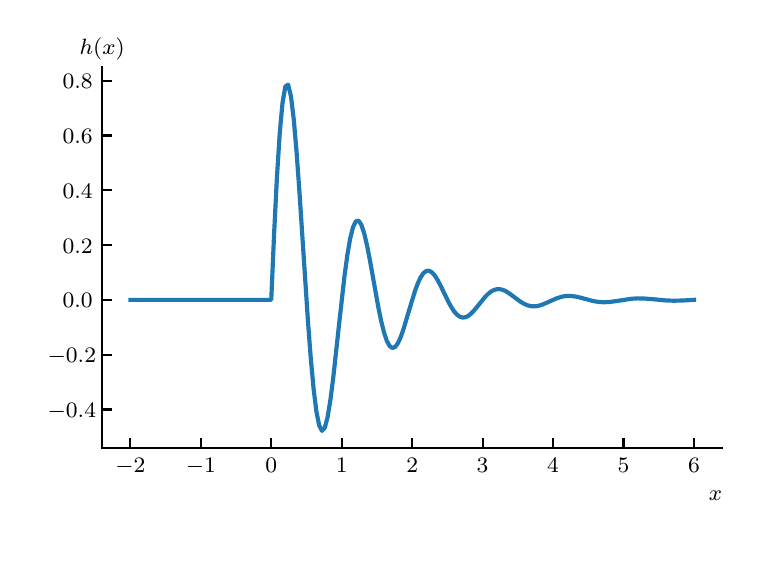
\begin{tikzpicture}%
\node[inner sep=0pt] {%% Creator: Matplotlib, PGF backend
%%
%% To include the figure in your LaTeX document, write
%%   \input{<filename>.pgf}
%%
%% Make sure the required packages are loaded in your preamble
%%   \usepackage{pgf}
%%
%% Also ensure that all the required font packages are loaded; for instance,
%% the lmodern package is sometimes necessary when using math font.
%%   \usepackage{lmodern}
%%
%% Figures using additional raster images can only be included by \input if
%% they are in the same directory as the main LaTeX file. For loading figures
%% from other directories you can use the `import` package
%%   \usepackage{import}
%%
%% and then include the figures with
%%   \import{<path to file>}{<filename>.pgf}
%%
%% Matplotlib used the following preamble
%%   \def\mathdefault#1{#1}
%%   \everymath=\expandafter{\the\everymath\displaystyle}
%%   \RequirePackage[T1]{fontenc}%
%%   \usepackage{newpxmath} % math font is Palatino compatible
%%   \let\Bbbk\relax % so it doesn't clash with amssymb
%%   \usepackage[no-math]{fontspec}
%%   \setmainfont{Palatino}
%%   \setmonofont{Latin Modern Mono}[%
%%   Scale=1.05, % a touch smaller than MatchLowercase
%%   BoldFont=*,
%%   BoldFeatures={FakeBold=2}
%%   ]
%%   \setsansfont{Helvetica}
%%   \renewcommand{\mathdefault}[1][]{}
%%   \usepackage{fontspec}
%%   \setmainfont{Palatino.ttc}[Path=\detokenize{/System/Library/Fonts/}]
%%   \setsansfont{DejaVuSans.ttf}[Path=\detokenize{/Users/ricopicone/anaconda3/envs/engcom/lib/python3.11/site-packages/matplotlib/mpl-data/fonts/ttf/}]
%%   \setmonofont{DejaVuSansMono.ttf}[Path=\detokenize{/Users/ricopicone/anaconda3/envs/engcom/lib/python3.11/site-packages/matplotlib/mpl-data/fonts/ttf/}]
%%   \makeatletter\@ifpackageloaded{underscore}{}{\usepackage[strings]{underscore}}\makeatother
%%
\begingroup%
\makeatletter%
\begin{pgfpicture}%
\pgfpathrectangle{\pgfpointorigin}{\pgfqpoint{3.572444in}{2.529415in}}%
\pgfusepath{use as bounding box, clip}%
\begin{pgfscope}%
\pgfsetbuttcap%
\pgfsetmiterjoin%
\definecolor{currentfill}{rgb}{1.000000,1.000000,1.000000}%
\pgfsetfillcolor{currentfill}%
\pgfsetlinewidth{0.000000pt}%
\definecolor{currentstroke}{rgb}{1.000000,1.000000,1.000000}%
\pgfsetstrokecolor{currentstroke}%
\pgfsetdash{}{0pt}%
\pgfpathmoveto{\pgfqpoint{0.000000in}{0.000000in}}%
\pgfpathlineto{\pgfqpoint{3.572444in}{0.000000in}}%
\pgfpathlineto{\pgfqpoint{3.572444in}{2.529415in}}%
\pgfpathlineto{\pgfqpoint{0.000000in}{2.529415in}}%
\pgfpathlineto{\pgfqpoint{0.000000in}{0.000000in}}%
\pgfpathclose%
\pgfusepath{fill}%
\end{pgfscope}%
\begin{pgfscope}%
\pgfsetbuttcap%
\pgfsetmiterjoin%
\definecolor{currentfill}{rgb}{1.000000,1.000000,1.000000}%
\pgfsetfillcolor{currentfill}%
\pgfsetlinewidth{0.000000pt}%
\definecolor{currentstroke}{rgb}{0.000000,0.000000,0.000000}%
\pgfsetstrokecolor{currentstroke}%
\pgfsetstrokeopacity{0.000000}%
\pgfsetdash{}{0pt}%
\pgfpathmoveto{\pgfqpoint{0.372444in}{0.427040in}}%
\pgfpathlineto{\pgfqpoint{3.472444in}{0.427040in}}%
\pgfpathlineto{\pgfqpoint{3.472444in}{2.330625in}}%
\pgfpathlineto{\pgfqpoint{0.372444in}{2.330625in}}%
\pgfpathlineto{\pgfqpoint{0.372444in}{0.427040in}}%
\pgfpathclose%
\pgfusepath{fill}%
\end{pgfscope}%
\begin{pgfscope}%
\pgfsetbuttcap%
\pgfsetroundjoin%
\definecolor{currentfill}{rgb}{0.000000,0.000000,0.000000}%
\pgfsetfillcolor{currentfill}%
\pgfsetlinewidth{0.803000pt}%
\definecolor{currentstroke}{rgb}{0.000000,0.000000,0.000000}%
\pgfsetstrokecolor{currentstroke}%
\pgfsetdash{}{0pt}%
\pgfsys@defobject{currentmarker}{\pgfqpoint{0.000000in}{0.000000in}}{\pgfqpoint{0.000000in}{0.048611in}}{%
\pgfpathmoveto{\pgfqpoint{0.000000in}{0.000000in}}%
\pgfpathlineto{\pgfqpoint{0.000000in}{0.048611in}}%
\pgfusepath{stroke,fill}%
}%
\begin{pgfscope}%
\pgfsys@transformshift{0.513353in}{0.427040in}%
\pgfsys@useobject{currentmarker}{}%
\end{pgfscope}%
\end{pgfscope}%
\begin{pgfscope}%
\definecolor{textcolor}{rgb}{0.000000,0.000000,0.000000}%
\pgfsetstrokecolor{textcolor}%
\pgfsetfillcolor{textcolor}%
\pgftext[x=0.513353in,y=0.378429in,,top]{\color{textcolor}{\rmfamily\fontsize{8.000000}{9.600000}\selectfont\catcode`\^=\active\def^{\ifmmode\sp\else\^{}\fi}\catcode`\%=\active\def%{\%}$\mathdefault{\ensuremath{-}2}$}}%
\end{pgfscope}%
\begin{pgfscope}%
\pgfsetbuttcap%
\pgfsetroundjoin%
\definecolor{currentfill}{rgb}{0.000000,0.000000,0.000000}%
\pgfsetfillcolor{currentfill}%
\pgfsetlinewidth{0.803000pt}%
\definecolor{currentstroke}{rgb}{0.000000,0.000000,0.000000}%
\pgfsetstrokecolor{currentstroke}%
\pgfsetdash{}{0pt}%
\pgfsys@defobject{currentmarker}{\pgfqpoint{0.000000in}{0.000000in}}{\pgfqpoint{0.000000in}{0.048611in}}{%
\pgfpathmoveto{\pgfqpoint{0.000000in}{0.000000in}}%
\pgfpathlineto{\pgfqpoint{0.000000in}{0.048611in}}%
\pgfusepath{stroke,fill}%
}%
\begin{pgfscope}%
\pgfsys@transformshift{0.865626in}{0.427040in}%
\pgfsys@useobject{currentmarker}{}%
\end{pgfscope}%
\end{pgfscope}%
\begin{pgfscope}%
\definecolor{textcolor}{rgb}{0.000000,0.000000,0.000000}%
\pgfsetstrokecolor{textcolor}%
\pgfsetfillcolor{textcolor}%
\pgftext[x=0.865626in,y=0.378429in,,top]{\color{textcolor}{\rmfamily\fontsize{8.000000}{9.600000}\selectfont\catcode`\^=\active\def^{\ifmmode\sp\else\^{}\fi}\catcode`\%=\active\def%{\%}$\mathdefault{\ensuremath{-}1}$}}%
\end{pgfscope}%
\begin{pgfscope}%
\pgfsetbuttcap%
\pgfsetroundjoin%
\definecolor{currentfill}{rgb}{0.000000,0.000000,0.000000}%
\pgfsetfillcolor{currentfill}%
\pgfsetlinewidth{0.803000pt}%
\definecolor{currentstroke}{rgb}{0.000000,0.000000,0.000000}%
\pgfsetstrokecolor{currentstroke}%
\pgfsetdash{}{0pt}%
\pgfsys@defobject{currentmarker}{\pgfqpoint{0.000000in}{0.000000in}}{\pgfqpoint{0.000000in}{0.048611in}}{%
\pgfpathmoveto{\pgfqpoint{0.000000in}{0.000000in}}%
\pgfpathlineto{\pgfqpoint{0.000000in}{0.048611in}}%
\pgfusepath{stroke,fill}%
}%
\begin{pgfscope}%
\pgfsys@transformshift{1.217899in}{0.427040in}%
\pgfsys@useobject{currentmarker}{}%
\end{pgfscope}%
\end{pgfscope}%
\begin{pgfscope}%
\definecolor{textcolor}{rgb}{0.000000,0.000000,0.000000}%
\pgfsetstrokecolor{textcolor}%
\pgfsetfillcolor{textcolor}%
\pgftext[x=1.217899in,y=0.378429in,,top]{\color{textcolor}{\rmfamily\fontsize{8.000000}{9.600000}\selectfont\catcode`\^=\active\def^{\ifmmode\sp\else\^{}\fi}\catcode`\%=\active\def%{\%}$\mathdefault{0}$}}%
\end{pgfscope}%
\begin{pgfscope}%
\pgfsetbuttcap%
\pgfsetroundjoin%
\definecolor{currentfill}{rgb}{0.000000,0.000000,0.000000}%
\pgfsetfillcolor{currentfill}%
\pgfsetlinewidth{0.803000pt}%
\definecolor{currentstroke}{rgb}{0.000000,0.000000,0.000000}%
\pgfsetstrokecolor{currentstroke}%
\pgfsetdash{}{0pt}%
\pgfsys@defobject{currentmarker}{\pgfqpoint{0.000000in}{0.000000in}}{\pgfqpoint{0.000000in}{0.048611in}}{%
\pgfpathmoveto{\pgfqpoint{0.000000in}{0.000000in}}%
\pgfpathlineto{\pgfqpoint{0.000000in}{0.048611in}}%
\pgfusepath{stroke,fill}%
}%
\begin{pgfscope}%
\pgfsys@transformshift{1.570171in}{0.427040in}%
\pgfsys@useobject{currentmarker}{}%
\end{pgfscope}%
\end{pgfscope}%
\begin{pgfscope}%
\definecolor{textcolor}{rgb}{0.000000,0.000000,0.000000}%
\pgfsetstrokecolor{textcolor}%
\pgfsetfillcolor{textcolor}%
\pgftext[x=1.570171in,y=0.378429in,,top]{\color{textcolor}{\rmfamily\fontsize{8.000000}{9.600000}\selectfont\catcode`\^=\active\def^{\ifmmode\sp\else\^{}\fi}\catcode`\%=\active\def%{\%}$\mathdefault{1}$}}%
\end{pgfscope}%
\begin{pgfscope}%
\pgfsetbuttcap%
\pgfsetroundjoin%
\definecolor{currentfill}{rgb}{0.000000,0.000000,0.000000}%
\pgfsetfillcolor{currentfill}%
\pgfsetlinewidth{0.803000pt}%
\definecolor{currentstroke}{rgb}{0.000000,0.000000,0.000000}%
\pgfsetstrokecolor{currentstroke}%
\pgfsetdash{}{0pt}%
\pgfsys@defobject{currentmarker}{\pgfqpoint{0.000000in}{0.000000in}}{\pgfqpoint{0.000000in}{0.048611in}}{%
\pgfpathmoveto{\pgfqpoint{0.000000in}{0.000000in}}%
\pgfpathlineto{\pgfqpoint{0.000000in}{0.048611in}}%
\pgfusepath{stroke,fill}%
}%
\begin{pgfscope}%
\pgfsys@transformshift{1.922444in}{0.427040in}%
\pgfsys@useobject{currentmarker}{}%
\end{pgfscope}%
\end{pgfscope}%
\begin{pgfscope}%
\definecolor{textcolor}{rgb}{0.000000,0.000000,0.000000}%
\pgfsetstrokecolor{textcolor}%
\pgfsetfillcolor{textcolor}%
\pgftext[x=1.922444in,y=0.378429in,,top]{\color{textcolor}{\rmfamily\fontsize{8.000000}{9.600000}\selectfont\catcode`\^=\active\def^{\ifmmode\sp\else\^{}\fi}\catcode`\%=\active\def%{\%}$\mathdefault{2}$}}%
\end{pgfscope}%
\begin{pgfscope}%
\pgfsetbuttcap%
\pgfsetroundjoin%
\definecolor{currentfill}{rgb}{0.000000,0.000000,0.000000}%
\pgfsetfillcolor{currentfill}%
\pgfsetlinewidth{0.803000pt}%
\definecolor{currentstroke}{rgb}{0.000000,0.000000,0.000000}%
\pgfsetstrokecolor{currentstroke}%
\pgfsetdash{}{0pt}%
\pgfsys@defobject{currentmarker}{\pgfqpoint{0.000000in}{0.000000in}}{\pgfqpoint{0.000000in}{0.048611in}}{%
\pgfpathmoveto{\pgfqpoint{0.000000in}{0.000000in}}%
\pgfpathlineto{\pgfqpoint{0.000000in}{0.048611in}}%
\pgfusepath{stroke,fill}%
}%
\begin{pgfscope}%
\pgfsys@transformshift{2.274717in}{0.427040in}%
\pgfsys@useobject{currentmarker}{}%
\end{pgfscope}%
\end{pgfscope}%
\begin{pgfscope}%
\definecolor{textcolor}{rgb}{0.000000,0.000000,0.000000}%
\pgfsetstrokecolor{textcolor}%
\pgfsetfillcolor{textcolor}%
\pgftext[x=2.274717in,y=0.378429in,,top]{\color{textcolor}{\rmfamily\fontsize{8.000000}{9.600000}\selectfont\catcode`\^=\active\def^{\ifmmode\sp\else\^{}\fi}\catcode`\%=\active\def%{\%}$\mathdefault{3}$}}%
\end{pgfscope}%
\begin{pgfscope}%
\pgfsetbuttcap%
\pgfsetroundjoin%
\definecolor{currentfill}{rgb}{0.000000,0.000000,0.000000}%
\pgfsetfillcolor{currentfill}%
\pgfsetlinewidth{0.803000pt}%
\definecolor{currentstroke}{rgb}{0.000000,0.000000,0.000000}%
\pgfsetstrokecolor{currentstroke}%
\pgfsetdash{}{0pt}%
\pgfsys@defobject{currentmarker}{\pgfqpoint{0.000000in}{0.000000in}}{\pgfqpoint{0.000000in}{0.048611in}}{%
\pgfpathmoveto{\pgfqpoint{0.000000in}{0.000000in}}%
\pgfpathlineto{\pgfqpoint{0.000000in}{0.048611in}}%
\pgfusepath{stroke,fill}%
}%
\begin{pgfscope}%
\pgfsys@transformshift{2.626990in}{0.427040in}%
\pgfsys@useobject{currentmarker}{}%
\end{pgfscope}%
\end{pgfscope}%
\begin{pgfscope}%
\definecolor{textcolor}{rgb}{0.000000,0.000000,0.000000}%
\pgfsetstrokecolor{textcolor}%
\pgfsetfillcolor{textcolor}%
\pgftext[x=2.626990in,y=0.378429in,,top]{\color{textcolor}{\rmfamily\fontsize{8.000000}{9.600000}\selectfont\catcode`\^=\active\def^{\ifmmode\sp\else\^{}\fi}\catcode`\%=\active\def%{\%}$\mathdefault{4}$}}%
\end{pgfscope}%
\begin{pgfscope}%
\pgfsetbuttcap%
\pgfsetroundjoin%
\definecolor{currentfill}{rgb}{0.000000,0.000000,0.000000}%
\pgfsetfillcolor{currentfill}%
\pgfsetlinewidth{0.803000pt}%
\definecolor{currentstroke}{rgb}{0.000000,0.000000,0.000000}%
\pgfsetstrokecolor{currentstroke}%
\pgfsetdash{}{0pt}%
\pgfsys@defobject{currentmarker}{\pgfqpoint{0.000000in}{0.000000in}}{\pgfqpoint{0.000000in}{0.048611in}}{%
\pgfpathmoveto{\pgfqpoint{0.000000in}{0.000000in}}%
\pgfpathlineto{\pgfqpoint{0.000000in}{0.048611in}}%
\pgfusepath{stroke,fill}%
}%
\begin{pgfscope}%
\pgfsys@transformshift{2.979262in}{0.427040in}%
\pgfsys@useobject{currentmarker}{}%
\end{pgfscope}%
\end{pgfscope}%
\begin{pgfscope}%
\definecolor{textcolor}{rgb}{0.000000,0.000000,0.000000}%
\pgfsetstrokecolor{textcolor}%
\pgfsetfillcolor{textcolor}%
\pgftext[x=2.979262in,y=0.378429in,,top]{\color{textcolor}{\rmfamily\fontsize{8.000000}{9.600000}\selectfont\catcode`\^=\active\def^{\ifmmode\sp\else\^{}\fi}\catcode`\%=\active\def%{\%}$\mathdefault{5}$}}%
\end{pgfscope}%
\begin{pgfscope}%
\pgfsetbuttcap%
\pgfsetroundjoin%
\definecolor{currentfill}{rgb}{0.000000,0.000000,0.000000}%
\pgfsetfillcolor{currentfill}%
\pgfsetlinewidth{0.803000pt}%
\definecolor{currentstroke}{rgb}{0.000000,0.000000,0.000000}%
\pgfsetstrokecolor{currentstroke}%
\pgfsetdash{}{0pt}%
\pgfsys@defobject{currentmarker}{\pgfqpoint{0.000000in}{0.000000in}}{\pgfqpoint{0.000000in}{0.048611in}}{%
\pgfpathmoveto{\pgfqpoint{0.000000in}{0.000000in}}%
\pgfpathlineto{\pgfqpoint{0.000000in}{0.048611in}}%
\pgfusepath{stroke,fill}%
}%
\begin{pgfscope}%
\pgfsys@transformshift{3.331535in}{0.427040in}%
\pgfsys@useobject{currentmarker}{}%
\end{pgfscope}%
\end{pgfscope}%
\begin{pgfscope}%
\definecolor{textcolor}{rgb}{0.000000,0.000000,0.000000}%
\pgfsetstrokecolor{textcolor}%
\pgfsetfillcolor{textcolor}%
\pgftext[x=3.331535in,y=0.378429in,,top]{\color{textcolor}{\rmfamily\fontsize{8.000000}{9.600000}\selectfont\catcode`\^=\active\def^{\ifmmode\sp\else\^{}\fi}\catcode`\%=\active\def%{\%}$\mathdefault{6}$}}%
\end{pgfscope}%
\begin{pgfscope}%
\definecolor{textcolor}{rgb}{0.000000,0.000000,0.000000}%
\pgfsetstrokecolor{textcolor}%
\pgfsetfillcolor{textcolor}%
\pgftext[x=3.472444in,y=0.211437in,right,top]{\color{textcolor}{\rmfamily\fontsize{8.000000}{9.600000}\selectfont\catcode`\^=\active\def^{\ifmmode\sp\else\^{}\fi}\catcode`\%=\active\def%{\%}$x$}}%
\end{pgfscope}%
\begin{pgfscope}%
\pgfsetbuttcap%
\pgfsetroundjoin%
\definecolor{currentfill}{rgb}{0.000000,0.000000,0.000000}%
\pgfsetfillcolor{currentfill}%
\pgfsetlinewidth{0.803000pt}%
\definecolor{currentstroke}{rgb}{0.000000,0.000000,0.000000}%
\pgfsetstrokecolor{currentstroke}%
\pgfsetdash{}{0pt}%
\pgfsys@defobject{currentmarker}{\pgfqpoint{0.000000in}{0.000000in}}{\pgfqpoint{0.048611in}{0.000000in}}{%
\pgfpathmoveto{\pgfqpoint{0.000000in}{0.000000in}}%
\pgfpathlineto{\pgfqpoint{0.048611in}{0.000000in}}%
\pgfusepath{stroke,fill}%
}%
\begin{pgfscope}%
\pgfsys@transformshift{0.372444in}{0.620602in}%
\pgfsys@useobject{currentmarker}{}%
\end{pgfscope}%
\end{pgfscope}%
\begin{pgfscope}%
\definecolor{textcolor}{rgb}{0.000000,0.000000,0.000000}%
\pgfsetstrokecolor{textcolor}%
\pgfsetfillcolor{textcolor}%
\pgftext[x=0.100000in, y=0.580183in, left, base]{\color{textcolor}{\rmfamily\fontsize{8.000000}{9.600000}\selectfont\catcode`\^=\active\def^{\ifmmode\sp\else\^{}\fi}\catcode`\%=\active\def%{\%}$\mathdefault{\ensuremath{-}0.4}$}}%
\end{pgfscope}%
\begin{pgfscope}%
\pgfsetbuttcap%
\pgfsetroundjoin%
\definecolor{currentfill}{rgb}{0.000000,0.000000,0.000000}%
\pgfsetfillcolor{currentfill}%
\pgfsetlinewidth{0.803000pt}%
\definecolor{currentstroke}{rgb}{0.000000,0.000000,0.000000}%
\pgfsetstrokecolor{currentstroke}%
\pgfsetdash{}{0pt}%
\pgfsys@defobject{currentmarker}{\pgfqpoint{0.000000in}{0.000000in}}{\pgfqpoint{0.048611in}{0.000000in}}{%
\pgfpathmoveto{\pgfqpoint{0.000000in}{0.000000in}}%
\pgfpathlineto{\pgfqpoint{0.048611in}{0.000000in}}%
\pgfusepath{stroke,fill}%
}%
\begin{pgfscope}%
\pgfsys@transformshift{0.372444in}{0.894592in}%
\pgfsys@useobject{currentmarker}{}%
\end{pgfscope}%
\end{pgfscope}%
\begin{pgfscope}%
\definecolor{textcolor}{rgb}{0.000000,0.000000,0.000000}%
\pgfsetstrokecolor{textcolor}%
\pgfsetfillcolor{textcolor}%
\pgftext[x=0.100000in, y=0.854173in, left, base]{\color{textcolor}{\rmfamily\fontsize{8.000000}{9.600000}\selectfont\catcode`\^=\active\def^{\ifmmode\sp\else\^{}\fi}\catcode`\%=\active\def%{\%}$\mathdefault{\ensuremath{-}0.2}$}}%
\end{pgfscope}%
\begin{pgfscope}%
\pgfsetbuttcap%
\pgfsetroundjoin%
\definecolor{currentfill}{rgb}{0.000000,0.000000,0.000000}%
\pgfsetfillcolor{currentfill}%
\pgfsetlinewidth{0.803000pt}%
\definecolor{currentstroke}{rgb}{0.000000,0.000000,0.000000}%
\pgfsetstrokecolor{currentstroke}%
\pgfsetdash{}{0pt}%
\pgfsys@defobject{currentmarker}{\pgfqpoint{0.000000in}{0.000000in}}{\pgfqpoint{0.048611in}{0.000000in}}{%
\pgfpathmoveto{\pgfqpoint{0.000000in}{0.000000in}}%
\pgfpathlineto{\pgfqpoint{0.048611in}{0.000000in}}%
\pgfusepath{stroke,fill}%
}%
\begin{pgfscope}%
\pgfsys@transformshift{0.372444in}{1.168582in}%
\pgfsys@useobject{currentmarker}{}%
\end{pgfscope}%
\end{pgfscope}%
\begin{pgfscope}%
\definecolor{textcolor}{rgb}{0.000000,0.000000,0.000000}%
\pgfsetstrokecolor{textcolor}%
\pgfsetfillcolor{textcolor}%
\pgftext[x=0.174333in, y=1.128164in, left, base]{\color{textcolor}{\rmfamily\fontsize{8.000000}{9.600000}\selectfont\catcode`\^=\active\def^{\ifmmode\sp\else\^{}\fi}\catcode`\%=\active\def%{\%}$\mathdefault{0.0}$}}%
\end{pgfscope}%
\begin{pgfscope}%
\pgfsetbuttcap%
\pgfsetroundjoin%
\definecolor{currentfill}{rgb}{0.000000,0.000000,0.000000}%
\pgfsetfillcolor{currentfill}%
\pgfsetlinewidth{0.803000pt}%
\definecolor{currentstroke}{rgb}{0.000000,0.000000,0.000000}%
\pgfsetstrokecolor{currentstroke}%
\pgfsetdash{}{0pt}%
\pgfsys@defobject{currentmarker}{\pgfqpoint{0.000000in}{0.000000in}}{\pgfqpoint{0.048611in}{0.000000in}}{%
\pgfpathmoveto{\pgfqpoint{0.000000in}{0.000000in}}%
\pgfpathlineto{\pgfqpoint{0.048611in}{0.000000in}}%
\pgfusepath{stroke,fill}%
}%
\begin{pgfscope}%
\pgfsys@transformshift{0.372444in}{1.442573in}%
\pgfsys@useobject{currentmarker}{}%
\end{pgfscope}%
\end{pgfscope}%
\begin{pgfscope}%
\definecolor{textcolor}{rgb}{0.000000,0.000000,0.000000}%
\pgfsetstrokecolor{textcolor}%
\pgfsetfillcolor{textcolor}%
\pgftext[x=0.174333in, y=1.402154in, left, base]{\color{textcolor}{\rmfamily\fontsize{8.000000}{9.600000}\selectfont\catcode`\^=\active\def^{\ifmmode\sp\else\^{}\fi}\catcode`\%=\active\def%{\%}$\mathdefault{0.2}$}}%
\end{pgfscope}%
\begin{pgfscope}%
\pgfsetbuttcap%
\pgfsetroundjoin%
\definecolor{currentfill}{rgb}{0.000000,0.000000,0.000000}%
\pgfsetfillcolor{currentfill}%
\pgfsetlinewidth{0.803000pt}%
\definecolor{currentstroke}{rgb}{0.000000,0.000000,0.000000}%
\pgfsetstrokecolor{currentstroke}%
\pgfsetdash{}{0pt}%
\pgfsys@defobject{currentmarker}{\pgfqpoint{0.000000in}{0.000000in}}{\pgfqpoint{0.048611in}{0.000000in}}{%
\pgfpathmoveto{\pgfqpoint{0.000000in}{0.000000in}}%
\pgfpathlineto{\pgfqpoint{0.048611in}{0.000000in}}%
\pgfusepath{stroke,fill}%
}%
\begin{pgfscope}%
\pgfsys@transformshift{0.372444in}{1.716563in}%
\pgfsys@useobject{currentmarker}{}%
\end{pgfscope}%
\end{pgfscope}%
\begin{pgfscope}%
\definecolor{textcolor}{rgb}{0.000000,0.000000,0.000000}%
\pgfsetstrokecolor{textcolor}%
\pgfsetfillcolor{textcolor}%
\pgftext[x=0.174333in, y=1.676144in, left, base]{\color{textcolor}{\rmfamily\fontsize{8.000000}{9.600000}\selectfont\catcode`\^=\active\def^{\ifmmode\sp\else\^{}\fi}\catcode`\%=\active\def%{\%}$\mathdefault{0.4}$}}%
\end{pgfscope}%
\begin{pgfscope}%
\pgfsetbuttcap%
\pgfsetroundjoin%
\definecolor{currentfill}{rgb}{0.000000,0.000000,0.000000}%
\pgfsetfillcolor{currentfill}%
\pgfsetlinewidth{0.803000pt}%
\definecolor{currentstroke}{rgb}{0.000000,0.000000,0.000000}%
\pgfsetstrokecolor{currentstroke}%
\pgfsetdash{}{0pt}%
\pgfsys@defobject{currentmarker}{\pgfqpoint{0.000000in}{0.000000in}}{\pgfqpoint{0.048611in}{0.000000in}}{%
\pgfpathmoveto{\pgfqpoint{0.000000in}{0.000000in}}%
\pgfpathlineto{\pgfqpoint{0.048611in}{0.000000in}}%
\pgfusepath{stroke,fill}%
}%
\begin{pgfscope}%
\pgfsys@transformshift{0.372444in}{1.990553in}%
\pgfsys@useobject{currentmarker}{}%
\end{pgfscope}%
\end{pgfscope}%
\begin{pgfscope}%
\definecolor{textcolor}{rgb}{0.000000,0.000000,0.000000}%
\pgfsetstrokecolor{textcolor}%
\pgfsetfillcolor{textcolor}%
\pgftext[x=0.174333in, y=1.950135in, left, base]{\color{textcolor}{\rmfamily\fontsize{8.000000}{9.600000}\selectfont\catcode`\^=\active\def^{\ifmmode\sp\else\^{}\fi}\catcode`\%=\active\def%{\%}$\mathdefault{0.6}$}}%
\end{pgfscope}%
\begin{pgfscope}%
\pgfsetbuttcap%
\pgfsetroundjoin%
\definecolor{currentfill}{rgb}{0.000000,0.000000,0.000000}%
\pgfsetfillcolor{currentfill}%
\pgfsetlinewidth{0.803000pt}%
\definecolor{currentstroke}{rgb}{0.000000,0.000000,0.000000}%
\pgfsetstrokecolor{currentstroke}%
\pgfsetdash{}{0pt}%
\pgfsys@defobject{currentmarker}{\pgfqpoint{0.000000in}{0.000000in}}{\pgfqpoint{0.048611in}{0.000000in}}{%
\pgfpathmoveto{\pgfqpoint{0.000000in}{0.000000in}}%
\pgfpathlineto{\pgfqpoint{0.048611in}{0.000000in}}%
\pgfusepath{stroke,fill}%
}%
\begin{pgfscope}%
\pgfsys@transformshift{0.372444in}{2.264544in}%
\pgfsys@useobject{currentmarker}{}%
\end{pgfscope}%
\end{pgfscope}%
\begin{pgfscope}%
\definecolor{textcolor}{rgb}{0.000000,0.000000,0.000000}%
\pgfsetstrokecolor{textcolor}%
\pgfsetfillcolor{textcolor}%
\pgftext[x=0.174333in, y=2.224125in, left, base]{\color{textcolor}{\rmfamily\fontsize{8.000000}{9.600000}\selectfont\catcode`\^=\active\def^{\ifmmode\sp\else\^{}\fi}\catcode`\%=\active\def%{\%}$\mathdefault{0.8}$}}%
\end{pgfscope}%
\begin{pgfscope}%
\definecolor{textcolor}{rgb}{0.000000,0.000000,0.000000}%
\pgfsetstrokecolor{textcolor}%
\pgfsetfillcolor{textcolor}%
\pgftext[x=0.372444in,y=2.368696in,,bottom]{\color{textcolor}{\rmfamily\fontsize{8.000000}{9.600000}\selectfont\catcode`\^=\active\def^{\ifmmode\sp\else\^{}\fi}\catcode`\%=\active\def%{\%}$h(x)$}}%
\end{pgfscope}%
\begin{pgfscope}%
\pgfpathrectangle{\pgfqpoint{0.372444in}{0.427040in}}{\pgfqpoint{3.100000in}{1.903585in}}%
\pgfusepath{clip}%
\pgfsetrectcap%
\pgfsetroundjoin%
\pgfsetlinewidth{1.505625pt}%
\definecolor{currentstroke}{rgb}{0.121569,0.466667,0.705882}%
\pgfsetstrokecolor{currentstroke}%
\pgfsetdash{}{0pt}%
\pgfpathmoveto{\pgfqpoint{0.513353in}{1.168582in}}%
\pgfpathlineto{\pgfqpoint{1.217899in}{1.168582in}}%
\pgfpathlineto{\pgfqpoint{1.231990in}{1.495917in}}%
\pgfpathlineto{\pgfqpoint{1.246081in}{1.777820in}}%
\pgfpathlineto{\pgfqpoint{1.260171in}{2.000333in}}%
\pgfpathlineto{\pgfqpoint{1.274262in}{2.154247in}}%
\pgfpathlineto{\pgfqpoint{1.288353in}{2.235308in}}%
\pgfpathlineto{\pgfqpoint{1.302444in}{2.244098in}}%
\pgfpathlineto{\pgfqpoint{1.316535in}{2.185630in}}%
\pgfpathlineto{\pgfqpoint{1.330626in}{2.068694in}}%
\pgfpathlineto{\pgfqpoint{1.344717in}{1.905026in}}%
\pgfpathlineto{\pgfqpoint{1.358808in}{1.708349in}}%
\pgfpathlineto{\pgfqpoint{1.401081in}{1.066503in}}%
\pgfpathlineto{\pgfqpoint{1.415171in}{0.880514in}}%
\pgfpathlineto{\pgfqpoint{1.429262in}{0.726659in}}%
\pgfpathlineto{\pgfqpoint{1.443353in}{0.611990in}}%
\pgfpathlineto{\pgfqpoint{1.457444in}{0.540595in}}%
\pgfpathlineto{\pgfqpoint{1.471535in}{0.513567in}}%
\pgfpathlineto{\pgfqpoint{1.485626in}{0.529166in}}%
\pgfpathlineto{\pgfqpoint{1.499717in}{0.583151in}}%
\pgfpathlineto{\pgfqpoint{1.513808in}{0.669228in}}%
\pgfpathlineto{\pgfqpoint{1.527899in}{0.779600in}}%
\pgfpathlineto{\pgfqpoint{1.556081in}{1.038133in}}%
\pgfpathlineto{\pgfqpoint{1.584262in}{1.289002in}}%
\pgfpathlineto{\pgfqpoint{1.598353in}{1.392708in}}%
\pgfpathlineto{\pgfqpoint{1.612444in}{1.474566in}}%
\pgfpathlineto{\pgfqpoint{1.626535in}{1.531188in}}%
\pgfpathlineto{\pgfqpoint{1.640626in}{1.561009in}}%
\pgfpathlineto{\pgfqpoint{1.654717in}{1.564242in}}%
\pgfpathlineto{\pgfqpoint{1.668808in}{1.542733in}}%
\pgfpathlineto{\pgfqpoint{1.682899in}{1.499715in}}%
\pgfpathlineto{\pgfqpoint{1.696990in}{1.439505in}}%
\pgfpathlineto{\pgfqpoint{1.711081in}{1.367151in}}%
\pgfpathlineto{\pgfqpoint{1.753353in}{1.131029in}}%
\pgfpathlineto{\pgfqpoint{1.767444in}{1.062608in}}%
\pgfpathlineto{\pgfqpoint{1.781535in}{1.006008in}}%
\pgfpathlineto{\pgfqpoint{1.795626in}{0.963824in}}%
\pgfpathlineto{\pgfqpoint{1.809717in}{0.937559in}}%
\pgfpathlineto{\pgfqpoint{1.823808in}{0.927616in}}%
\pgfpathlineto{\pgfqpoint{1.837899in}{0.933354in}}%
\pgfpathlineto{\pgfqpoint{1.851990in}{0.953214in}}%
\pgfpathlineto{\pgfqpoint{1.866081in}{0.984880in}}%
\pgfpathlineto{\pgfqpoint{1.880171in}{1.025484in}}%
\pgfpathlineto{\pgfqpoint{1.908353in}{1.120593in}}%
\pgfpathlineto{\pgfqpoint{1.936535in}{1.212882in}}%
\pgfpathlineto{\pgfqpoint{1.950626in}{1.251034in}}%
\pgfpathlineto{\pgfqpoint{1.964717in}{1.281148in}}%
\pgfpathlineto{\pgfqpoint{1.978808in}{1.301978in}}%
\pgfpathlineto{\pgfqpoint{1.992899in}{1.312948in}}%
\pgfpathlineto{\pgfqpoint{2.006990in}{1.314138in}}%
\pgfpathlineto{\pgfqpoint{2.021081in}{1.306225in}}%
\pgfpathlineto{\pgfqpoint{2.035171in}{1.290399in}}%
\pgfpathlineto{\pgfqpoint{2.049262in}{1.268249in}}%
\pgfpathlineto{\pgfqpoint{2.063353in}{1.241632in}}%
\pgfpathlineto{\pgfqpoint{2.105626in}{1.154767in}}%
\pgfpathlineto{\pgfqpoint{2.119717in}{1.129597in}}%
\pgfpathlineto{\pgfqpoint{2.133808in}{1.108774in}}%
\pgfpathlineto{\pgfqpoint{2.147899in}{1.093256in}}%
\pgfpathlineto{\pgfqpoint{2.161990in}{1.083594in}}%
\pgfpathlineto{\pgfqpoint{2.176081in}{1.079936in}}%
\pgfpathlineto{\pgfqpoint{2.190171in}{1.082047in}}%
\pgfpathlineto{\pgfqpoint{2.204262in}{1.089353in}}%
\pgfpathlineto{\pgfqpoint{2.218353in}{1.101002in}}%
\pgfpathlineto{\pgfqpoint{2.232444in}{1.115939in}}%
\pgfpathlineto{\pgfqpoint{2.288808in}{1.184879in}}%
\pgfpathlineto{\pgfqpoint{2.302899in}{1.198915in}}%
\pgfpathlineto{\pgfqpoint{2.316990in}{1.209993in}}%
\pgfpathlineto{\pgfqpoint{2.331081in}{1.217656in}}%
\pgfpathlineto{\pgfqpoint{2.345171in}{1.221691in}}%
\pgfpathlineto{\pgfqpoint{2.359262in}{1.222129in}}%
\pgfpathlineto{\pgfqpoint{2.373353in}{1.219218in}}%
\pgfpathlineto{\pgfqpoint{2.387444in}{1.213396in}}%
\pgfpathlineto{\pgfqpoint{2.401535in}{1.205248in}}%
\pgfpathlineto{\pgfqpoint{2.429717in}{1.184753in}}%
\pgfpathlineto{\pgfqpoint{2.457899in}{1.163500in}}%
\pgfpathlineto{\pgfqpoint{2.471990in}{1.154240in}}%
\pgfpathlineto{\pgfqpoint{2.486081in}{1.146580in}}%
\pgfpathlineto{\pgfqpoint{2.500171in}{1.140871in}}%
\pgfpathlineto{\pgfqpoint{2.514262in}{1.137317in}}%
\pgfpathlineto{\pgfqpoint{2.528353in}{1.135971in}}%
\pgfpathlineto{\pgfqpoint{2.542444in}{1.136748in}}%
\pgfpathlineto{\pgfqpoint{2.556535in}{1.139435in}}%
\pgfpathlineto{\pgfqpoint{2.570626in}{1.143721in}}%
\pgfpathlineto{\pgfqpoint{2.598808in}{1.155488in}}%
\pgfpathlineto{\pgfqpoint{2.641081in}{1.174578in}}%
\pgfpathlineto{\pgfqpoint{2.669262in}{1.183816in}}%
\pgfpathlineto{\pgfqpoint{2.683353in}{1.186635in}}%
\pgfpathlineto{\pgfqpoint{2.697444in}{1.188120in}}%
\pgfpathlineto{\pgfqpoint{2.711535in}{1.188281in}}%
\pgfpathlineto{\pgfqpoint{2.739717in}{1.185068in}}%
\pgfpathlineto{\pgfqpoint{2.767899in}{1.178469in}}%
\pgfpathlineto{\pgfqpoint{2.824262in}{1.163306in}}%
\pgfpathlineto{\pgfqpoint{2.852444in}{1.158388in}}%
\pgfpathlineto{\pgfqpoint{2.880626in}{1.156585in}}%
\pgfpathlineto{\pgfqpoint{2.908808in}{1.157860in}}%
\pgfpathlineto{\pgfqpoint{2.936990in}{1.161458in}}%
\pgfpathlineto{\pgfqpoint{3.021535in}{1.174187in}}%
\pgfpathlineto{\pgfqpoint{3.049717in}{1.175770in}}%
\pgfpathlineto{\pgfqpoint{3.077899in}{1.175435in}}%
\pgfpathlineto{\pgfqpoint{3.120171in}{1.172219in}}%
\pgfpathlineto{\pgfqpoint{3.190626in}{1.165605in}}%
\pgfpathlineto{\pgfqpoint{3.232899in}{1.164169in}}%
\pgfpathlineto{\pgfqpoint{3.275171in}{1.165218in}}%
\pgfpathlineto{\pgfqpoint{3.331535in}{1.168582in}}%
\pgfpathlineto{\pgfqpoint{3.331535in}{1.168582in}}%
\pgfusepath{stroke}%
\end{pgfscope}%
\begin{pgfscope}%
\pgfsetrectcap%
\pgfsetmiterjoin%
\pgfsetlinewidth{0.803000pt}%
\definecolor{currentstroke}{rgb}{0.000000,0.000000,0.000000}%
\pgfsetstrokecolor{currentstroke}%
\pgfsetdash{}{0pt}%
\pgfpathmoveto{\pgfqpoint{0.372444in}{0.427040in}}%
\pgfpathlineto{\pgfqpoint{0.372444in}{2.330625in}}%
\pgfusepath{stroke}%
\end{pgfscope}%
\begin{pgfscope}%
\pgfsetrectcap%
\pgfsetmiterjoin%
\pgfsetlinewidth{0.803000pt}%
\definecolor{currentstroke}{rgb}{0.000000,0.000000,0.000000}%
\pgfsetstrokecolor{currentstroke}%
\pgfsetdash{}{0pt}%
\pgfpathmoveto{\pgfqpoint{0.372444in}{0.427040in}}%
\pgfpathlineto{\pgfqpoint{3.472444in}{0.427040in}}%
\pgfusepath{stroke}%
\end{pgfscope}%
\end{pgfpicture}%
\makeatother%
\endgroup%
};%
\end{tikzpicture}%
\caption{}
\label{fig:publishing_with_makefile-figure-2}
\end{figure}

\phantomsection\label{44e76862}
\nointerlineskip\nointerlineskip\begin{minted}[autogobble,samepage]{python}
plt.show()
\end{minted}
